\documentclass{article}

% \DeclareUnicodeCharacter{202F}{~}
% if you need to pass options to natbib, use, e.g.:
%     \PassOptionsToPackage{numbers, compress}{natbib}
% before loading neurips_2025
% \usepackage{neurips_2026}
% the "default" option is equal to the "main" option, which is used for the Main Track with double-blind reviewing.
% 1. "main" option is used for the Main Track
%  \usepackage[main]{neurips_2026}
% 2. "position" option is used for the Position Paper Track
%  \usepackage[position]{neurips_2026}
% 3. "eandd" option is used for the Evaluations & Datasets Track
 % \usepackage[eandd]{neurips_2026}
 % if you want to opt-in for a de-anomymized submission (not recommended, but OK):
 %\usepackage[eandd, nonanonymous]{neurips_2026}
% 4. "creativeai" option is used for the Creative AI Track
%  \usepackage[creativeai]{neurips_2026}
% 5. "sglblindworkshop" option is used for the Workshop with single-blind reviewing
 % \usepackage[sglblindworkshop]{neurips_2026}
% 6. "dblblindworkshop" option is used for the Workshop with double-blind reviewing
%  \usepackage[dblblindworkshop]{neurips_2026}

% After being accepted, the authors should add "final" behind the track to compile a camera-ready version.
% 1. Main Track
 % \usepackage[main, final]{neurips_2026}
% 2. Position Paper Track
%  \usepackage[position, final]{neurips_2026}
% 3. Evaluations & Datasets Track
 % \usepackage[eandd, final]{neurips_2026}
% 4. Creative AI Track
%  \usepackage[creativeai, final]{neurips_2026}
% 5. Workshop with single-blind reviewing
%  \usepackage[sglblindworkshop, final]{neurips_2026}
% 6. Workshop with double-blind reviewing
%  \usepackage[dblblindworkshop, final]{neurips_2026}
% Note. For the workshop paper template, both \title{} and \workshoptitle{} are required, with the former indicating the paper title shown in the title and the latter indicating the workshop title displayed in the footnote.
% For workshops (5., 6.), the authors should add the name of the workshop, "\workshoptitle" command is used to set the workshop title.
% \workshoptitle{WORKSHOP TITLE}

% "preprint" option is used for arXiv or other preprint submissions
 \usepackage[preprint]{neurips_2026}

% to avoid loading the natbib package, add option nonatbib:
%    \usepackage[nonatbib]{neurips_2026}

\usepackage[utf8]{inputenc} % allow utf-8 input
\usepackage[T1]{fontenc}    % use 8-bit T1 fonts
\usepackage{hyperref}       % hyperlinks
\usepackage{url}            % simple URL typesetting
\usepackage{booktabs}       % professional-quality tables
\usepackage{amsfonts}       % blackboard math symbols
\usepackage{nicefrac}       % compact symbols for 1/2, etc.
\usepackage{microtype}      % microtypography
\usepackage{xcolor}  
\usepackage{multirow}
\usepackage{enumitem}
\usepackage{amsmath,amssymb,amsthm}
\usepackage{graphicx}
\usepackage{wrapfig}
\usepackage{subcaption}

%%%%%%%%%%%%%%%%%%%%%%%%%%%%%%%%
% THEOREMS
%%%%%%%%%%%%%%%%%%%%%%%%%%%%%%%%
\theoremstyle{plain}
\newtheorem{theorem}{Theorem}[section]
\newtheorem{proposition}[theorem]{Proposition}
\newtheorem{lemma}[theorem]{Lemma}
\newtheorem{corollary}[theorem]{Corollary}
\theoremstyle{definition}
\newtheorem{definition}[theorem]{Definition}
\newtheorem{assumption}[theorem]{Assumption}
\theoremstyle{remark}
\newtheorem{remark}[theorem]{Remark}
\theoremstyle{problem}
\newtheorem{problem}[theorem]{Problem}

\title{SOMA: Efficient Multi-turn LLM Serving via Small Language Model}

% \author{%
%   Xueqi Cheng\\
%   % Department of Computer Science\\
%   Florida State University University\\
%   % Pittsburgh, PA 15213 \\
%   \texttt{xc25@fsu.edu} \\
%   % examples of more authors
%   \And
%   Qiong Wu \\
%   AT\&T Chief Data Office  \\
%   % Address \\
%   \texttt{qw6547@att.com} \\
%   \And
%   Zhengyi Zhou \\
%   AT\&T Chief Data Office  \\
%   % Address \\
%   \texttt{zz547k@att.com} \\
%   \And
%   Xugui Zhou \\
%   Louisiana State University \\
%   % Address \\
%   \texttt{xuguizhou@lsu.edu } \\
%   \And
%   Tyler Derr \\
%   Vanderbilt University \\
%   % Address \\
%   \texttt{tyler.derr@vanderbilt.edu} \\
% \And
%   Yushun Dong \\
%   Florida State University University \\
%   % Address \\
%   \texttt{yushun.dong@fsu.edu} \\
% }

\author{%
\begin{tabular}{c}
\small
\textbf{Xueqi Cheng}$^{1}$ \quad
\textbf{Qiong Wu}$^{2}$ \quad
\textbf{Zhengyi Zhou}$^{2}$ \quad
\textbf{Xugui Zhou}$^{3}$ \quad
\textbf{Tyler Derr}$^{4}$ \quad
\textbf{Yushun Dong}$^{1}$ \\
{\normalfont\footnotesize
$^{1}$Florida State University \quad
$^{2}$AT\&T Chief Data Office \quad
$^{3}$Louisiana State University \quad
$^{4}$Vanderbilt University} \\
{\normalfont\ttfamily\scriptsize
\{xc25,yushun.dong\}@fsu.edu;\ \{qw6547,zz547k\}@att.com} \
{\normalfont\ttfamily\scriptsize
xuguizhou@lsu.edu;\ tyler.derr@vanderbilt.edu}
\end{tabular}%
}


\newcommand{\xq}[1]{{\color{red}{#1}}}

\begin{document}
\maketitle

% ============================================================
\begin{abstract}

Large Language Models (LLMs) are increasingly deployed in multi-turn dialogue settings where preserving conversational context across turns is essential. A standard serving practice concatenates the full dialogue history at every turn, which reliably maintains coherence but incurs substantial cost in latency, memory, and API expenditure, especially when queries are routed to large proprietary models. Existing approaches often struggle to balance the trade-off between response quality and efficiency. We propose a framework that exploits the early turns of a session to estimate a local response manifold and then adapt a smaller surrogate model to this local region for the remainder of the conversation. Concretely, we learn soft prompts that maximize semantic divergence between the large and surrogate small language models' responses to surface least-aligned local directions, stabilize training with anti-degeneration control, and distill the mined cases into localized LoRA fine-tuning so the surrogate runs without prompts at inference. A simple gate enables a one-time switch with rollback on drift. We further provide a theoretical analysis for key components in SOMA. Extensive experiments show the effectiveness of SOMA. The source code is provided at: 
% \url{https://anonymous.4open.science/r/SOMA-4175}.
\url{https://github.com/LabRAI/SOMA}.
\end{abstract}



\section{Introduction}\label{sec:intro} 




% \yd{expensive - mitigate expensive existing works are not good - our observations and this observation gives us a very unique and interesting opportunity (i.e., to local estimate it) but directly use is not good - we propose a framework which is wonderful}



Large language models (LLMs) such as the GPT series~\citep{radford2019language, brown2020language, achiam2023gpt}, LLaMA~\citep{touvron2023llama}, Claude~\citep{anthropic_introducing_claude_2023}, and DeepSeek~\citep{guo2025deepseek} have demonstrated strong performance in real-world machine-learning-as-a-service (MLaaS) applications, ranging from chat assistants to code generation~\citep{park2023thinking, dong2023towards, liu2024exploring, li2026llmclinicalgraphstructure, yu2026health}. As LLMs are increasingly deployed interactively, \textit{multi-turn LLM serving}, which covers extended interactions between humans and LLMs or among LLM agents, has become a key research focus~\citep{yi2024survey, li2025beyond, zhao2025amplifying}.
However, supporting efficient context-dependent 
% \yd{is this word some terminology in this domain? why do we need to put it here?} 
% \xq{yes, they mean we need whole history to process the later turns for LLM, but since I mention stateless later, I will just remove it}
multi-turn interaction remains a key challenge, as most LLM serving systems are stateless and require resending the entire conversation history, including all prior queries and responses, with each new query to generate a new response~\citep{ananda2025beyond, moon2025accelerating}. This leads to redundant computation, high latency, and rising serving costs as conversations lengthen.

Previous work has explored efficient multi-turn LLM serving through two main approaches. One line of work focuses on \textit{single-model methods} that compress dialogue history~\citep{wang2025recursively, chen2024compress, xiao2024efficient}, retrieve memory from external modules~\citep{melz2023enhancing, gutierrez2024hipporag}, or reuse attention computations~\citep{gao2024cost, jeong2025accelerating, anthropic_prompt_caching_2024}. However, these still rely heavily on large LLMs for every turn, leading to high monetary cost, latency, and GPU usage. They also often truncate or overlook extended context, limiting reasoning over long dialogues. Another line adopts \textit{multi-model methods}, routing simple queries to smaller models while escalating harder ones to larger LLMs~\citep{behera2025towards, schick2023toolformer, ding2024hybrid, shnitzer2023large}. Yet, small models struggle to generalize across dialogue complexity, and model switching introduces additional overhead. Moreover, LLMs are known to rely on early turns~\citep{xiao2024efficient, laban2025llms}, compounding the difficulty of maintaining coherence. 
% \yd{I think we did involve both types of baselines into our experiments, right? make sure the answer is yes and do a call back in experimental setup when introducing baselines like ``there are mainly two mainstreams of models xxx" (of course also mention your straightforward methods there as well)} Recognizing these limitations, we ask: 
%\xq{sure}
% \yd{i changed the ``design" to ``achieve" since only designing something is still NOT what people want.}\xq{sure}
% \yd{your question should be whether something is possible, not whether ``you/we" can achieve xx. People care about what the nature allows, not what ``you/we" can do.}

\textit{\textbf{Is it possible to achieve an efficient, context-aware multi-turn LLM serving framework that avoids recomputing the full history at every turn while preserving response quality?}}


% \yd{mention to achieve this goal, we perform in-depth explorations, and it reveals xxx. Plus, I think the logic in this paragraph is unnecessarily complex. follow: to handle gap, we explored more - reveal phenomenon - this phenomenon really makes sense with real-world examples - intuitively, directly dealing with the short turns with a small model can improve efficiency - but we still need to make it context-relevant, i.e., to make it aware of the context contained in the big head - mention existing strategies and mention they are not good and mention this is really difficult}
To answer this question, we examine real-world multi-turn dialogues across domains and find a long-tail distribution of token counts over turns: early turns are substantially longer, while later turns shrink. This phenomenon aligns with the intuition of prior work that early turns typically carry \rev{the substantive openings that set the issues and anchors of a conversation}, including questions, requests, and proposals, while later turns are typically minimal acknowledgments~\citep{he2018decoupling, stolcke2000dialogue}.
% \yd{mention this phenomenon aligns with our intuition of how people typically interacting with the model} 
This long-tail trend gives rise to an intuitive idea: since later turns are relatively short, a smaller language model might suffice to generate responses more cost-efficiently. 
% \yd{starting from here, we involved some irrelevant redundant logic. simply say that the problem comes from the big head: if small models still need to process the head, efficiency is still a problem.} 
The bottleneck, however, is the “big head”: most grounding is established early, and later turns remain highly dependent on it. A small model may behave reasonably at the start, but its responses drift from the large model as the dialogue progresses, so simply handing later turns to a small model degrades quality. The small model must therefore not only process shorter inputs but also approximate the larger model's behavior within the local region of its output space that the prior dialogue induces. We call this a local manifold approximation problem.

Building on these insights, we present SOMA (\textit{S}oft-prompts for l\textit{O}cal \textit{M}anifold \textit{A}pproximation), which adapts a small language model to the local behavior of a large one, conditioned on the early turns of a session, through a three-stage pipeline: (1) \textit{soft-prompt tuning}, which explores the local region induced by the early context to find the directions of maximal behavioral divergence between the two models; (2) \textit{localized fine-tuning}, which aligns the small model with the large one on a handful of mined input--output pairs; and (3) \textit{efficient inference}, which serves later turns from a compressed context and rolls back to the large model when the topic drifts. Our contributions are: 
% \yd{your contributions are too detailed. do this: 1 - Explorations revealing the phenomenon of xxx; 2 - Novel framework for xxx; 3 - Theoretical analysis of xxx; 3 - empirical evaluation for xxx. 4 in total.}
% \yd{name each with textbf bold font. make all exactly 2-rows or 3-rows}
\begin{itemize}[left=0pt,itemsep=2pt]
\item \textbf{Long-tail pattern in multi-turn dialogues.} 
We reveal an under-explored long-tail pattern in multi-turn dialogues: the first few turns concentrate heavy context, while later turns are shorter yet more dependent on earlier ones. This suggests large savings if a small, cheap model can serve the later turns once it is given the accumulated context.

% (The separate "Empirical characterization" point is merged above per feedback.)

% \item \textbf{Empirical characterization.} \yd{we shall remove this -- merge this one into the previous one very briefly would be good enough}
% We quantify tail heaviness across multiple datasets and show strong context reliance as conversations progress. The measurements reveal that a small language model could potentially replace a large language model during the conversation to serve later turns. This empirical characterization suggests that a small model can replace a 

\item \textbf{SOMA: Efficient multi-turn serving.} It first learns soft prompts that expose the largest surrogate–original response dissimilarity, then adapts the surrogate localized LoRA accordingly, enabling prompt-free inference with a simple cosine gate for switching and rollback.

\item \textbf{Theory analysis and empirical evaluation.} 
We provide concentration-based bounds for switching, coverage guarantees for prompt-direction search, and suboptimality limits for selected directions. Guided by these results, empirical studies show the effectiveness of SOMA in real world.
\end{itemize}


% \yd{no need to do this any more. We shall remove this paragraph. We are tight on page limit.}
% The paper is structured as follows: Section~\ref{sec:prelim} introduces preliminaries and empirically characterizes the long-tail token–turn pattern in multi-turn dialogues. Section~\ref{sec:method} presents details of SOMA, including soft-prompt mining to expose least-aligned directions, localized LoRA fine-tuning to adapt the surrogate, and efficiency-aware inference with switching and rollback. Section~\ref{sec:theory} develops the theoretical foundations, including warm-start generalization and detection bounds for switching as well as coverage guarantees for prompt-direction search. Section~\ref{sec:exp} reports empirical experiment results across six datasets. Section~\ref{sec:conclusion} concludes the work.







\section{Preliminaries}\label{sec:prelim}

\subsection{Notations}

A multi-turn dialogue prefix of length $k$ is $\mathcal{D}_k=\{(q_1,a_1),\ldots,(q_k,a_k)\}$, where $q_t$ is the user query at turn $t$ and $a_t$ is the model response. We write $F$ for the original model, a proprietary black-box LLM as is common in machine-learning-as-a-service (MLaaS), and $G$ for the small surrogate. The textual response of model $M\in\{F,G\}$ at turn $t$ is $a_t^M$. Let $f_M(\cdot)$ map an input sequence to the hidden space, so that $\mathbf{h}_t=f_M(q_{\le t})\in\mathbb{R}^d$ is the hidden state at turn $t$; the first $k$ hidden states $\mathcal{H}_k=\{\mathbf{h}_1,\ldots,\mathbf{h}_k\}$ induce a local region $\mathcal{M}_k^M\subset\mathbb{R}^d$. A soft prompt of length $L$ is a matrix $\mathbf{P}\in\mathbb{R}^{L\times d}$. Appendix~\ref{sec:notation} lists all symbols.

\subsection{Exploring Token--Turn Patterns in Multi-Turn LLM Dialogues}
\label{sec:long_tail}

Standard serving processes each new request together with the entire history, so the cost of a turn grows with the length of the conversation. The amount of \emph{new} information in a turn, however, need not grow at all. We therefore first study token usage across turns.


We consider four representative settings: \textit{ShareGPT}~\citep{chen2024sharegpt4v} for open-ended human--LLM chat, \textit{ReMeDi}~\citep{yan2022remedi} for doctor--patient consultation, \textit{Craigslist Bargain}~\citep{he2018decoupling} for negotiation, and \textit{Multi-Character}~\citep{agentlans_multi-character_dialogue_2024} for multi-party role-play. Together they cover different speaker roles, task goals, and interaction structures. For each dataset, we compute the average token count at turn \(t\) and normalize it by the average of Turn~1.

\begin{wrapfigure}[13]{r}{0.42\textwidth}
  \vspace{-11pt}
  \centering
  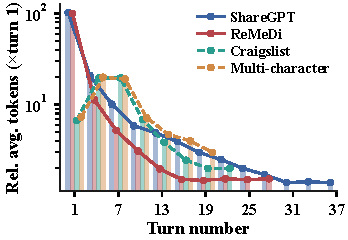
\includegraphics[width=0.419\textwidth]{figure/long_tail.pdf}
  \vspace{-18pt}
  \caption{Average token count per turn, normalized by Turn~1, on four dialogue datasets: usage drops after the early turns and forms a long tail.}
  \vspace{-11pt}
  \label{fig:longtail-token-decay}
\end{wrapfigure}
Figure~\ref{fig:longtail-token-decay} shows a consistent long-tail pattern. Early turns are token-heavy: they introduce the task, the topic, the constraints, and the speaker's intent. Later turns are much shorter and settle at a low, stable level. Shorter does not mean independent. Many later turns read as local updates to a dialogue state that has already been established, so the marginal new input shrinks while standard serving keeps re-processing the full prefix. This mismatch motivates an adaptive strategy: let the original model establish the early dialogue state, and hand subsequent turns to a cheaper surrogate for as long as they stay within that state, instead of recomputing the full history.

\subsection{Local Manifold Approximation for Multi-Turn Dialogues}

The long-tail pattern creates an opportunity for surrogate serving, but a naive substitution is unreliable. A later turn is short precisely because much of its meaning is supplied by the preceding dialogue, so a surrogate that is not aligned with the original model under that prefix produces fluent responses that quietly drift from the intended context.

We describe this challenge through a local manifold view. Given a prefix \(\mathcal{D}_{k}\), the original model \(F\) and the surrogate \(G\) each induce a local region in their contextual representation space, and this region captures the current topic, constraints, style, and task state. The goal is to make the surrogate's region match that of the original model under the same prefix.

\begin{problem}[Local Manifold Approximation for Multi-Turn Interactions]
Given a dialogue prefix \(\mathcal{D}_{k}\) and an original model \(F\), learn a surrogate model \(G\in\mathcal{G}\) whose local representation region matches that of \(F\) under the same prefix:
\[
\min_{G\in\mathcal{G}}
\mathrm{dist}\!\left(
\mathcal{M}^{G}_{k}(\mathcal{D}_{k}),
\mathcal{M}^{F}_{k}(\mathcal{D}_{k})
\right),
\]
where \(\mathcal{M}^{F}_{k}(\mathcal{D}_{k})\) and \(\mathcal{M}^{G}_{k}(\mathcal{D}_{k})\) denote the local representation regions induced by the prefix, and \(\mathrm{dist}(\cdot,\cdot)\) measures their discrepancy.
\end{problem}

This formulation leads directly to SOMA. The early turns are used to expose where the surrogate disagrees with the original model within the current dialogue state, and these locally informative examples are then used to adapt the surrogate. After adaptation, the surrogate serves later turns only while the dialogue remains close to the learned region; when the conversation drifts, the system returns to the original model and refreshes the local state.

\section{SOMA: Local Manifold Approximation via Soft Prompts}\label{sec:method}

SOMA combines three components to enable efficient local serving. First, the original model \(F\) handles early turns to establish the dialogue state. Second, soft-prompt mining identifies where the surrogate \(G\) is least aligned with \(F\), and these hard local cases are distilled into a lightweight LoRA adapter. Third, a semantic gate switches to \(G\) only when local alignment is sufficient, while a drift detector rolls back to \(F\) when the dialogue moves away from the learned local state.

\subsection{Initialization}

We initialize a soft prompt matrix $\mathbf{P}\in\mathbb{R}^{L_p\times d}$ on the surrogate $G$. Each row is sampled i.i.d. from $\boldsymbol{p}_{\ell}\sim\mathcal{N}(\boldsymbol{0},\sigma^2\mathbf{I}_d)$, where $\sigma>0$ is the initialization scale. Let $\mathbf{E}=[\boldsymbol e_v]_{v\in\mathcal V}\in\mathbb{R}^{d\times |\mathcal V|}$ be the surrogate embedding matrix and let $\mathrm{tok}(v)$ denote the token string associated with index $v$.

Because the original model $F$ cannot accept continuous embedding vectors, the soft prompt is used in two aligned forms. The surrogate receives $\mathbf{P}$ directly at the embedding layer, while the original model receives a nearest-neighbor verbalization of the same prompt:
\[
v_{\ell}=\arg\max_{v\in\mathcal V}
\frac{\langle \boldsymbol p_{\ell},\boldsymbol e_v\rangle}{\|\boldsymbol p_{\ell}\|_2\|\boldsymbol e_v\|_2},
\qquad
V(\mathbf P)=\big(\mathrm{tok}(v_1),\ldots,\mathrm{tok}(v_{L_p})\big).
\]
Let $\mathcal D_{t-1}$ denote the text history before turn $t$ and let $q_t$ be the user query. During prompt mining, the two models are probed under comparable text conditioning:
\[
a_t^{F}=F\!\left(V(\mathbf P)\oplus\mathcal D_{t-1}\oplus q_t\right),
\qquad
 a_t^{G}=G\!\left(\mathbf P\oplus_{\mathrm{emb}}
\mathbf E(\mathrm{tok}_G(\mathcal D_{t-1}\oplus q_t))\right).
\]
Here $\mathrm{tok}_G(\cdot)$ is the tokenizer of $G$, $\mathbf E(\cdot)$ maps text tokens to embeddings, and $\oplus_{\mathrm{emb}}$ concatenates along the sequence dimension. This construction lets $F$ and $G$ be compared under the same dialogue state while allowing gradients to flow only through $\mathbf P$ on $G$.

\subsection{Soft Prompt Tuning for Mining Weak Alignment Directions}

We learn $\mathbf P$ by minimizing a differentiable objective that makes $G$ move away from $F$ on the local dialogue context. The objective has three components: a token-level semantic divergence loss, an expectation-weighted distribution-level divergence term, and an anti-degeneration regularizer.

\textbf{Semantic divergence loss.}
We use an unlikelihood-style loss~\citep{welleck2019neural} to discourage $G$ from assigning high probability to the tokens produced by $F$. A purely exact-token penalty is too narrow, since the surrogate could avoid the teacher token while still assigning high probability to close paraphrases. We therefore define a semantic neighborhood in the surrogate embedding space.

\begin{definition}[Semantic Neighborhood]
For token $u\in\mathcal V$, let $\mathcal N_k(u)$ be the set of the $k$ tokens in $\mathcal V\setminus\{u\}$ whose embeddings have the largest cosine similarity to $\boldsymbol e_u$.
\end{definition}

At turn $t$, the original model produces text $a_t^F$. We tokenize this text using the surrogate tokenizer,
$\boldsymbol y_t^F=\mathrm{tok}_G(a_t^F)=(y_{t,1}^F,\ldots,y_{t,T_F(t)}^F)$, so that the teacher output and surrogate distribution are expressed in the same vocabulary. For each teacher token, we assign temperature-weighted mass to the token and its embedding neighbors:
\[
s_{\tau}(v\mid y_{t,i}^F)=
\frac{\exp(\cos(\boldsymbol e_v,\boldsymbol e_{y_{t,i}^F})/\tau)}
{\sum_{u\in\{y_{t,i}^F\}\cup\mathcal N_k(y_{t,i}^F)}
\exp(\cos(\boldsymbol e_u,\boldsymbol e_{y_{t,i}^F})/\tau)},
\qquad \tau>0 .
\]
Let $S_t=\mathcal D_{t-1}\oplus q_t$. With causal masking, a single forward pass of $G$ on the prefix $S_t$ and the teacher answer prefix gives the next-token distributions
$\{\Pi_{t,i}(\mathbf P)\}_{i=1}^{T_F(t)}$, where
$\Pi_{t,i}(\mathbf P)=\pi_G(\cdot\mid S_t;\mathbf P, a_{t,<i}^F)$.
The semantic divergence loss is
\begin{equation}
\label{eq:sem-with-aF}
\mathcal L_{\mathrm{sem}}(\mathbf P;\mathcal D_{t-1},q_t)=
\frac{1}{T_F(t)}\sum_{i=1}^{T_F(t)}
\sum_{v\in\{y_{t,i}^F\}\cup\mathcal N_k(y_{t,i}^F)}
s_{\tau}(v\mid y_{t,i}^F)
\Big[-\log\big(1-\Pi_{t,i}(\mathbf P)[v]\big)\Big].
\end{equation}
Minimizing Eq.~\ref{eq:sem-with-aF} searches for prompts that expose local disagreement between $F$ and $G$ not only on exact tokens but also on nearby semantic alternatives.

\textbf{Expectation-weighted semantic divergence.}
The token-neighborhood loss may still miss distribution-level alignment: $G$ can reduce probability on a teacher token and its nearest neighbors while spreading mass over many other tokens with similar meaning. To detect this case, we compare the expected embedding of the surrogate's next-token distribution with the embedding of the teacher token. Since $\mathbf E\in\mathbb R^{d\times |\mathcal V|}$ stores token embeddings as columns, the expected embedding at position $i$ is $\bar{\boldsymbol e}_{t,i}=\mathbf E\Pi_{t,i}(\mathbf P)
=\sum_{v\in\mathcal V}\Pi_{t,i}(\mathbf P)[v] \boldsymbol e_v $. We upweight the neighborhood penalty when this expected embedding still points toward the teacher token $w_{t,i}(\mathbf P)=1+\lambda_{\mathrm{exp}}\,
\mathrm{clip}\!\left(
\cos(\bar{\boldsymbol e}_{t,i},\boldsymbol e_{y_{t,i}^{F}}),0,1
\right)$, where $\lambda_{\mathrm{exp}}\ge 0 $. The final semantic mining loss is then:
\begin{equation}
\label{eq:semexp-with-aF}
\mathcal L_{\mathrm{sem\_exp}}(\mathbf P;\mathcal D_{t-1},q_t)=
\frac{1}{T_F(t)}\sum_{i=1}^{T_F(t)}
w_{t,i}(\mathbf P)
\sum_{v\in\{y_{t,i}^F\}\cup\mathcal N_k(y_{t,i}^F)}
s_{\tau}(v\mid y_{t,i}^{F})
\Big[-\log\big(1-\Pi_{t,i}(\mathbf P)[v]\big)\Big].
\end{equation}
Thus the loss blocks local copying through the neighborhood term and detects broader semantic shadowing through the expectation weight.

\begin{theorem}[Directional Recovery]
\label{thm:dir_recovery}
Let \(\mathbf C=\mathbb E[\mathbf J^\top \mathbf J]\) be the local discrepancy Fisher matrix of \(G\) over the warm-start window, where \(\mathbf J\) is the Jacobian of \(G\)'s log next-token probabilities with respect to the soft prompt \(\mathbf P\). If the local discrepancy is smooth and approximately rank \(r\), then optimizing Eq.~\ref{eq:semexp-with-aF} recovers prompt directions whose span covers at least a \((1-\varepsilon)\) fraction of the top-\(r\) eigenmass of \(\mathbf C\), with smaller \(\varepsilon\) under better warm-start and neighborhood coverage.
\end{theorem}

\textbf{Anti-degeneration regularizer.}
Soft-prompt mining can collapse if $G$ assigns excessive probability to a few high-frequency tokens, producing repetitive or bland continuations that are uninformative about where $F$ and $G$ differ~\citep{li2023repetition,holtzman2019curious,meister2023locally}. We therefore preserve entropy near the prompt-context boundary. Reusing the logits from the same forward pass, define
\[
H_{\mathrm{tail}}(\mathbf P;t)=
\frac{1}{K}\sum_{i\in\mathrm{tail}(t,K)}
\left[-\sum_{v\in\mathcal V}\Pi_{t,i}(\mathbf P)[v]
\log \Pi_{t,i}(\mathbf P)[v]\right].
\]
The complete prompt-mining objective for a minibatch of warm-start turns $\mathcal B$ is
\begin{equation}
\label{eq:prompt-final}
\mathcal J(\mathbf P)=
\frac{1}{|\mathcal B|}\sum_{t\in\mathcal B}
\left[
\mathcal L_{\mathrm{sem\_exp}}(\mathbf P;\mathcal D_{t-1},q_t)
-\beta H_{\mathrm{tail}}(\mathbf P;t)
\right]
+\lambda_P\|\mathbf P\|_F^2 .
\end{equation}
We minimize Eq.~\ref{eq:prompt-final} with AdamW while freezing all weights of $G$. Gradient clipping stabilizes the prompt scale. For efficiency, semantic neighbors are retrieved using an ANN index over normalized token embeddings, and $\bar{\boldsymbol e}_{t,i}$ is computed with a top-$m$ truncation of $\Pi_{t,i}(\mathbf P)$ rather than a dense sum over the full vocabulary. The per-step overhead is therefore linear in the number of teacher-prefix positions and scales with $k+m$ rather than $|\mathcal V|$.

\subsection{Localized Fine-Tuning, Switching, and Rollback}

The learned soft prompts are session-local mining tools. After mining, SOMA converts them into ordinary local supervision for LoRA adaptation. For each warm-start turn, we score its hardness by the largest mined divergence $r_t=\max_{\mathbf P\in\mathcal P_{\mathrm{cand}}}
\mathcal L_{\mathrm{sem\_exp}}(\mathbf P;\mathcal D_{t-1},q_t)$ and form a local training set $\mathcal H$ from the highest-scoring turns and their original-model responses. This makes the data-mining role of soft prompts explicit: Random-FT trains on randomly selected local turns, whereas SOMA trains on turns selected because prompt mining exposes weak alignment directions.

We freeze the base weights of $G$, attach LoRA~\citep{hu2022lora} to attention and MLP projections, and optimize
\begin{equation}
\label{eq:lora-ft}
\mathcal L_{\mathrm{FT}}(\boldsymbol\Theta_{\mathrm{LoRA}})=
\frac{1}{|\mathcal H|}\sum_{(S_t,a_t^F)\in\mathcal H}
\omega_t\,\mathrm{NLL}\big(a_t^F\mid G(S_t;\boldsymbol\Theta_{\mathrm{LoRA}})\big),
\qquad
\omega_t\propto r_t .
\end{equation}
The continuous soft prompts are discarded after this stage. Thus, once SOMA switches, the online serving path uses only the LoRA-adapted surrogate and a compressed text context.

Before switching, SOMA verifies that the adapted surrogate \(G\) is both output-aligned and context-local: it requires high response similarity to the original model \(F\) on a small acceptance batch and checks that the current query remains close to the warm-start dialogue centroid. Once accepted, SOMA serves later turns using a compressed input \(\widetilde S_t\), which keeps a fixed-budget summary of earlier content together with the most recent \(K\) turns, avoiding repeated full-history processing. During surrogate serving, SOMA continuously monitors semantic drift; if recent queries move away from the learned local state, it rolls back to \(F\), refreshes the local summary and centroid, and switches back to \(G\) only after the acceptance gate passes again.
\section{Theoretical Analysis}\label{sec:theory}

This section answers two design questions: when SOMA may accept the session-local surrogate, and when its warm-start overhead is amortized. \rev{Both answers assume that later turns stay tied to the warm-start state, though not that they are easier. The results describe when SOMA can operate and claim no advantage over other mining strategies. Appendix~\ref{sec:app_proof} has the proofs and a candidate bound.}

\subsection{Switching Criterion}\label{sec:warm-start}

At turn $t$, with shared context $S_t=\mathcal D_{t-1}\oplus q_t$, we measure the discrepancy of the adapted surrogate with the bounded score $\mathsf{Gap}_{\Theta}(S_t)\in[0,1]$ of Section~\ref{sec:prelim}, where $\Theta$ is the current adapter. \rev{Since consecutive turns are dependent, we model per-turn statistics as an $m$-dependent sequence and use the effective sample sizes $W_{\mathrm{eff}}=W/(m+1)$ for the warm-start window and $|B|_{\mathrm{eff}}=|B|/(m+1)$ for an acceptance batch $B$. Lemma~\ref{lem:warmstart} shows that, with probability at least $1-\delta$, a bounded warm-start statistic lies within $\eta_W(\delta)=\sqrt{\log(2/\delta)/(2W_{\mathrm{eff}})}$ of its mean, so strongly dependent early turns may need a longer warm start before the switch can be assessed.}

\rev{The fidelity gate evaluates the adapted surrogate on an acceptance batch $B$ through its average gap $\widehat{\mathsf G}_B=\frac{1}{|B|}\sum_{S_j\in B}\mathsf{Gap}_{\Theta}(S_j)$, and the surrogate passes when $\widehat{\mathsf G}_B$ is below a threshold $\varepsilon$.}

\begin{proposition}[Acceptance Bound for Switching]\label{thm:detection}
\rev{Assume that warm-start and later states share the distribution $\mathcal Q_k$ (the locality premise of Section~\ref{sec:prelim}), let $B$ be drawn from it and be disjoint from the turns used to fit $\Theta$, and let $\gamma_B(\delta)=\sqrt{\log(1/\delta)/(2|B|_{\mathrm{eff}})}$. With probability at least $1-\delta$, $\mathbb E_{S\sim\mathcal Q_k}[\mathsf{Gap}_{\Theta}(S)]\le\widehat{\mathsf G}_B+\gamma_B(\delta)$. Hence $\widehat{\mathsf G}_B\le\varepsilon-\gamma_B(\delta)$ certifies $\mathbb E[\mathsf{Gap}_{\Theta}]\le\varepsilon$.}
\end{proposition}

\rev{A union bound combines the two results (Corollary~\ref{cor:switch}). An abrupt topic change typically fails the locality gate and triggers an immediate rollback to $F$. The guarantee has two practical limits. It needs a held-out acceptance batch, but our implementation reuses the warm-start turns for adaptation and acceptance, so in the reported experiments the gate works as a heuristic check. The bound is also loose. With $\delta=0.05$ and $|B|=24$, $\gamma_B\approx0.25$, which exceeds the thresholds $\varepsilon\in[0.05,0.12]$ themselves, so we set these thresholds empirically (Appendix~\ref{sec:app_proof}).}

\subsection{Net Efficiency Gain}\label{sec:theory-cost}

Because SOMA pays its warm-start overhead once, its efficiency must be judged per session. Let $T$ be the number of turns, $W$ the switch point, and $c_F(\cdot)$ and $c_G(\cdot)$ the per-turn costs (latency, tokens, or price) of $F$ and of $G$ on its compressed input $\widetilde S_t$; the net gain over serving every turn with $F$ is
\begin{equation}
\label{eq:net-gain}
\Delta C(T;W)=\sum_{t=W+1}^{T}\Big[c_F(\mathcal D_{t-1}\oplus q_t)-c_G(\widetilde S_t)\Big]
-C_{\mathrm{probe}}(W)-C_{\mathrm{LoRA}}(W)-C_{\mathrm{rb}}(T;W),
\end{equation}
where $C_{\mathrm{probe}}$ and $C_{\mathrm{LoRA}}$ are the mining and adaptation costs and $C_{\mathrm{rb}}$ covers drift checks and rollback; SOMA pays off only when the accumulated post-switch savings exceed this one-time overhead. \rev{This is consistent with Figure~\ref{fig:operating}(a), where sessions of 1--4 turns do not benefit and locally coherent sessions of 5 or more turns recover the initialization cost.}

\section{Empirical Studies of the Effectiveness of SOMA}\label{sec:exp}

We evaluate SOMA through five questions. \textbf{RQ1}: Can a small surrogate preserve the original model's responses? \textbf{RQ2}: Does higher response similarity also improve task-grounded quality? \textbf{RQ3}: When does SOMA provide net efficiency gains after warm-start and adaptation overhead? \textbf{RQ4}: Which components of SOMA are most important? \textbf{RQ5}: When is session-local serving reliable, and when should SOMA fall back to the large model?

\textbf{Datasets.} We evaluate SOMA on six multi-turn benchmarks: ShareGPT~\citep{chen2024sharegpt4v}, ReMeDi~\citep{yan2022remedi}, Craigslist~\citep{he2018decoupling}, Multi-Char~\citep{agentlans_multi-character_dialogue_2024}, MATH~\citep{hendrycks2021measuring}, and MT-Bench~\citep{zheng2023judging}. Dataset details and the context-dependence filtering are in Appendix~\ref{sec:app_dataset}.

\textbf{Models and baselines.} We test two model families: LLaMA, using LLaMA-3.1-70B as \(F\) and LLaMA-2-7B as \(G\), and Qwen, using Qwen-3-8B as \(F\) and Qwen-3-0.6B as \(G\). We compare with Original, Surrogate, History-Prefix, History-FT, LLMLingua-2~\citep{pan2024llmlingua}, and RouteLLM~\citep{ong2024routellmlearningroutellms}; Appendix~\ref{sec:app_baseline} details each baseline.

\textbf{Metrics.} We mainly measure teacher-fidelity similarity, i.e., how closely each method preserves the original model's response, using three LLM judges: GPT-OSS~\citep{openai2025gptoss120bgptoss20bmodel}, DeepSeek-V3, and Gemma-2-27B. To complement similarity with task-grounded quality, we report EM accuracy on MATH. Efficiency is measured by token usage, throughput, and end-to-end \rev{wall-clock} latency, \rev{which for SOMA includes soft-prompt mining, LoRA adaptation, and gating. All models run on vLLM~0.10.2 with automatic prefix caching, so every baseline reuses the KV cache across turns.}

\textbf{Implementation.} We set the warm-start window, acceptance batch, candidate count, and switch threshold from Section~\ref{sec:theory}; after switching, SOMA performs no further LoRA updates and keeps only the drift check. Appendix~\ref{sec:app_implementation} lists all hyperparameters.

\subsection{Experimental Results}
\label{sec:exp_res}

\paragraph{\textbf{RQ1: Response similarity to the original model.}}

\begin{table}[!t]
\centering
\caption{Response similarity to the original model on the LLaMA family. Higher is better. \rev{SOMA stays closest to the original model on all six datasets. It raises the average from 75.1 for the unadapted surrogate to 93.1, 0.9 points above the strongest baseline, RouteLLM.}}
\label{tab:llama-pct}
\resizebox{0.96\textwidth}{!}{
\begin{tabular}{lccccccc}
\toprule
 & \textbf{ShareGPT} & \textbf{ReMeDi} & \textbf{Craigslist} & \textbf{Multi-Char} & \textbf{MATH} & \textbf{MT-Bench} & \textbf{Avg.} \\
\midrule
Surrogate      & 79.2 $\pm$ 2.18 & 82.7 $\pm$ 1.95 & 74.3 $\pm$ 2.36 & 70.8 $\pm$ 1.73 & 66.2 $\pm$ 2.91 & 77.5 $\pm$ 2.04 & 75.1 $\pm$ 5.98 \\
History-Prefix & 86.1 $\pm$ 1.67 & 87.9 $\pm$ 1.55 & 82.4 $\pm$ 1.72 & 84.7 $\pm$ 1.69 & 80.3 $\pm$ 3.83 & 87.2 $\pm$ 1.58 & 84.8 $\pm$ 2.94 \\
History-FT     & 93.4 $\pm$ 2.12 & 91.8 $\pm$ 2.09 & 90.3 $\pm$ 1.23 & 89.1 $\pm$ 2.23 & 87.6 $\pm$ 2.26 & 92.4 $\pm$ 1.14 & 90.8 $\pm$ 2.18 \\
LLMLingua-2    & 84.6 $\pm$ 1.72 & 86.4 $\pm$ 1.63 & 80.8 $\pm$ 1.91 & 82.9 $\pm$ 1.58 & 78.1 $\pm$ 2.77 & 85.3 $\pm$ 1.66 & 83.0 $\pm$ \rev{3.11} \\
RouteLLM       & 95.3 $\pm$ 1.44 & 92.5 $\pm$ 1.07 & 91.0 $\pm$ 1.86 & 91.4 $\pm$ 1.23 & 89.6 $\pm$ 1.95 & 93.2 $\pm$ 1.12 & 92.2 $\pm$ \rev{1.98} \\
\midrule
\textbf{SOMA}  & \textbf{96.4 $\pm$ 1.91} & \textbf{93.2 $\pm$ 0.98} & \textbf{91.9 $\pm$ 2.49} & \textbf{92.3 $\pm$ 1.05} & \textbf{90.7 $\pm$ 1.12} & \textbf{94.1 $\pm$ 0.91} & \textbf{93.1 $\pm$ 1.99} \\
\bottomrule
\end{tabular}}
\vspace{-3mm}
\end{table}

\begin{table}[!t]
\centering
\caption{Response similarity to the original model on the Qwen family. Higher is better. \rev{SOMA again leads on all six datasets. Similarities are lower than for LLaMA, probably because the size gap is wider, and SOMA's average gain over the unadapted surrogate grows to 27.1 points.}}
\label{tab:qwen-pct}
\resizebox{0.96\textwidth}{!}{
\begin{tabular}{lccccccc}
\toprule
 & \textbf{ShareGPT} & \textbf{ReMeDi} & \textbf{Craigslist} & \textbf{Multi-Char} & \textbf{MATH} & \textbf{MT-Bench} & \textbf{Avg.} \\
\midrule
Surrogate       & 50.9 $\pm$ 1.21 & 63.5 $\pm$ 2.87 & 48.2 $\pm$ 3.40 & 44.7 $\pm$ 3.54 & 42.6 $\pm$ 1.70 & 40.4 $\pm$ 0.81 & 48.4 $\pm$ 8.31 \\
History-Prefix  & 70.5 $\pm$ 1.15 & 75.7 $\pm$ 2.01 & 63.0 $\pm$ 2.23 & 65.5 $\pm$ 0.91 & 51.3 $\pm$ 2.45 & 53.6 $\pm$ 2.32 & 63.3 $\pm$ 9.47 \\
History-FT      & 76.4 $\pm$ 1.68 & 79.2 $\pm$ 2.61 & 74.5 $\pm$ 3.56 & 63.2 $\pm$ 1.74 & 65.9 $\pm$ 1.70 & 62.7 $\pm$ 0.72 & 70.3 $\pm$ 7.23 \\
LLMLingua-2     & 68.9 $\pm$ 1.32 & 74.1 $\pm$ 2.14 & 61.2 $\pm$ 2.67 & 63.4 $\pm$ 1.18 & 49.8 $\pm$ 2.03 & 51.7 $\pm$ 1.45 & 61.5 $\pm$ \rev{9.49} \\
RouteLLM        & 79.6 $\pm$ 1.04 & 81.9 $\pm$ 1.36 & 75.1 $\pm$ 2.91 & 72.8 $\pm$ 1.62 & 67.3 $\pm$ 1.21 & 68.0 $\pm$ 0.96 & 74.1 $\pm$ \rev{5.95} \\
\midrule
\textbf{SOMA}   & \textbf{81.0 $\pm$ 0.93} & \textbf{83.2 $\pm$ 1.21} & \textbf{76.4 $\pm$ 3.85} & \textbf{74.2 $\pm$ 2.53} & \textbf{68.7 $\pm$ 1.28} & \textbf{69.2 $\pm$ 1.08} & \textbf{75.5 $\pm$ 5.97} \\
\bottomrule
\end{tabular}}
\vspace{-3mm}
\end{table}

\begin{table}[!t]
\centering
\caption{MATH exact-match accuracy. \rev{SOMA stays below the original model but recovers 77--78\% of the gap between the surrogate and the original model and outperforms every other baseline.}}
\label{tab:math-em}
\resizebox{\textwidth}{!}{
\begin{tabular}{lcccccc}
\toprule
\textbf{Family} & \textbf{Orig.} & \textbf{Surr.} & \textbf{Hist.-P} & \textbf{Hist.-FT} & \textbf{Route} & \textbf{SOMA} \\
\midrule
LLaMA & 48.34 $\pm$ 0.32 & 19.20 $\pm$ 0.78 & 25.03 $\pm$ 0.94 & 31.46 $\pm$ 0.87 & 33.88 $\pm$ 0.79 & \textbf{41.62 $\pm$ 0.66} \\
Qwen  & 36.48 $\pm$ 0.41 & 11.73 $\pm$ 0.64 & 16.21 $\pm$ 0.79 & 22.57 $\pm$ 0.83 & 25.08 $\pm$ 0.71 & \textbf{31.14 $\pm$ 0.74} \\
\bottomrule
\end{tabular}}
\vspace{-3mm}
\end{table}

After the warm-start stage, the surrogate should preserve the original model's behavior within the current dialogue state. Table~\ref{tab:llama-pct} reports response similarity on the LLaMA family. SOMA achieves the highest average similarity across all six datasets. The gap over Surrogate shows the behavior loss caused by directly replacing the large model with a smaller model. The gap over History-FT shows that local adaptation helps, \rev{and seems to help more when the warm-start turns are weighted by their anchoring scores.} The largest gains appear on MATH and Multi-Char, where later turns depend on accumulated reasoning states, constraints, and roles. \rev{Table~\ref{tab:qwen-pct} repeats the evaluation on the Qwen family. Absolute similarities are lower, likely because the capacity gap between Qwen-3-8B and Qwen-3-0.6B is wider and local imitation becomes harder. SOMA is still the best method on every dataset.}

\paragraph{\textbf{RQ2: Task-grounded quality.}}
Response similarity is the primary metric for replacing the original model, but similarity alone does not guarantee task quality. We therefore evaluate MATH using exact-match accuracy. Table~\ref{tab:math-em} shows that SOMA remains below the original large model, as expected, but substantially narrows the gap between the surrogate and the original model. SOMA also outperforms History-Prefix, History-FT, and RouteLLM in both model families. Thus SOMA's gains are not only surface-level matching: local adaptation also preserves more of the original model's reasoning.

\paragraph{\textbf{RQ3: End-to-end efficiency.}}

\begin{figure}[!t]
\centering
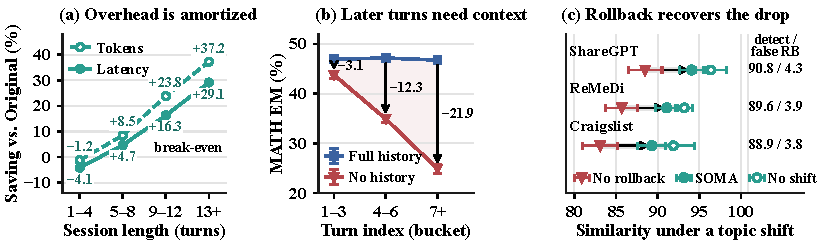
\includegraphics[width=\textwidth]{figure/operating.pdf}
\vspace{-5mm}
\caption{Operating range and reliability. (a) End-to-end saving of SOMA over Original on ShareGPT after all warm-start and adaptation overhead, by session length. (b) MATH exact match with and without the dialogue history: later turns remain context-dependent. (c) Response similarity under an abrupt topic shift without rollback, with SOMA's drift-aware rollback, and without a shift; the right column lists SOMA's shift-detection and false-rollback (RB) rates in \%.}
\label{fig:operating}
\vspace{-3mm}
\end{figure}

\begin{figure}[!t]
  \centering
  \begin{subfigure}[t]{0.49\textwidth}
    \centering
    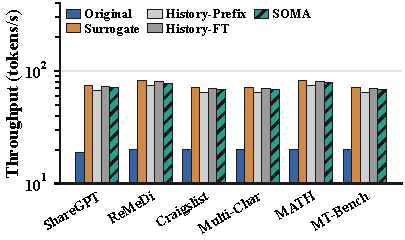
\includegraphics[width=\linewidth]{figure/llama_through.pdf}
    \caption{LLaMA family.}
  \end{subfigure}\hfill
  \begin{subfigure}[t]{0.49\textwidth}
    \centering
    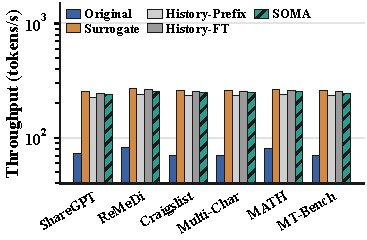
\includegraphics[width=\linewidth]{figure/qwen_through.pdf}
    \caption{Qwen family.}
  \end{subfigure}
  \vspace{-2mm}
  \caption{Throughput across six datasets. SOMA keeps the serving path close to the surrogate while maintaining higher similarity to the original model.}
  \label{fig:app_throughput}
\vspace{-3mm}
\end{figure}

SOMA reduces post-switch cost by serving the adapted surrogate with compressed context, but it also introduces one-time costs from soft-prompt probing and LoRA adaptation. Thus, the key question is whether the total session cost decreases after this overhead is included. SOMA reduces average token usage by avoiding repeated full-history serving after switching (Appendix~\ref{sec:app_eff}). Figure~\ref{fig:operating}(a) further shows the amortized operating range: \rev{SOMA is slightly unfavorable for sessions of 1--4 turns ($-4.1\%$ latency) and roughly breaks even at 5--8 turns ($+4.7\%$). From 9 turns on, it saves $16.3\%$ to $29.1\%$ latency and $23.8\%$ to $37.2\%$ tokens.} This matches SOMA's intended use case as an amortized serving strategy for conversations where enough later turns remain local to the warm-start state. \rev{Figure~\ref{fig:app_throughput} reports throughput on all six datasets for both families. SOMA runs at 95--97\% of the throughput of Surrogate and History-FT, about 5.6\% faster than History-Prefix and 3.1--3.9$\times$ faster than Original. Appendix~\ref{sec:app_eff} lists the per-dataset token costs.}

\paragraph{\textbf{RQ4: Component contributions.}}

We first ablate SOMA on the LLaMA family to identify which components drive the gains. Figure~\ref{fig:llama_ablation} shows that full SOMA performs best across all datasets. Removing the anti-degeneration loss consistently reduces performance, showing that entropy regularization keeps prompt mining stable and prevents collapsed, low-diversity soft prompts. Removing both the expectation-weighted term and the anti-degeneration loss leads to a larger drop, especially on harder datasets. \rev{This result suggests that the anchoring scores are most informative when the probe is both stable and semantic.} \rev{Figure~\ref{fig:qwen_ablation} repeats the ablation on the Qwen family and finds the same ordering, so the conclusion does not appear to hinge on the backbone. Figure~\ref{fig:mt_radar} breaks MT-Bench-101 down by ability for the LLaMA family. Relative to the surrogate, SOMA gains most on reasoning, reflection, and questioning, and it also improves understanding, interference handling, memory, and rephrasing to a smaller degree.}

% \begin{figure}[t]
%   \centering
%   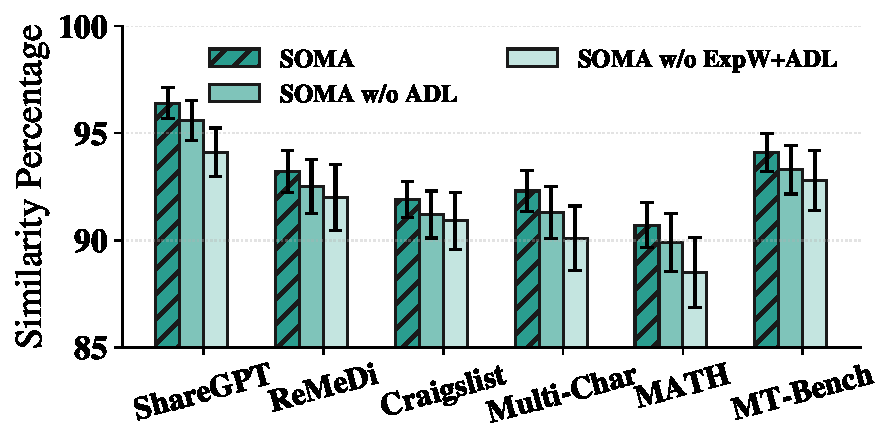
\includegraphics[width=0.70\textwidth]{figure/ablation_llama.pdf}
%   \caption{Ablation study on the LLaMA family. Full SOMA performs best, confirming the importance of anti-degeneration regularization and expectation-weighted divergence in soft-prompt mining.}
%   \label{fig:ablation-llama}
% \end{figure}

\paragraph{\textbf{RQ5: Reliability and fallback.}}

\begin{figure}[!t]
  \centering
  \begin{subfigure}[t]{0.344\textwidth}
    \centering
    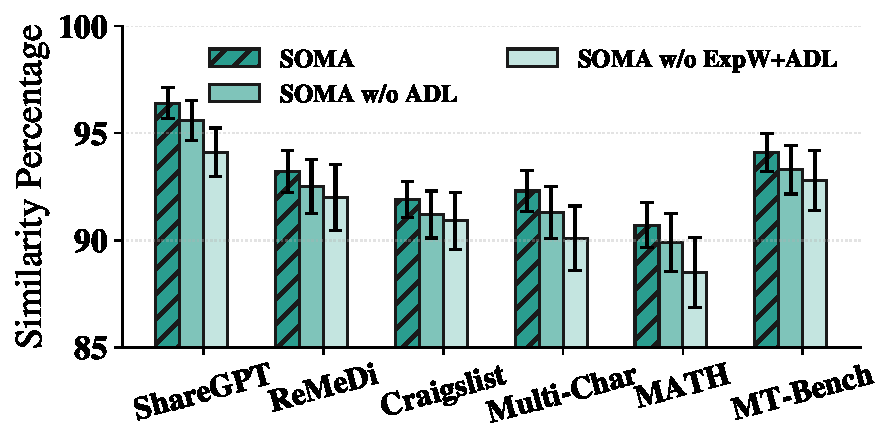
\includegraphics[width=\linewidth]{figure/ablation_llama.pdf}
    \caption{LLaMA ablation.}
    \label{fig:llama_ablation}
  \end{subfigure}\hfill
  \begin{subfigure}[t]{0.344\textwidth}
    \centering
    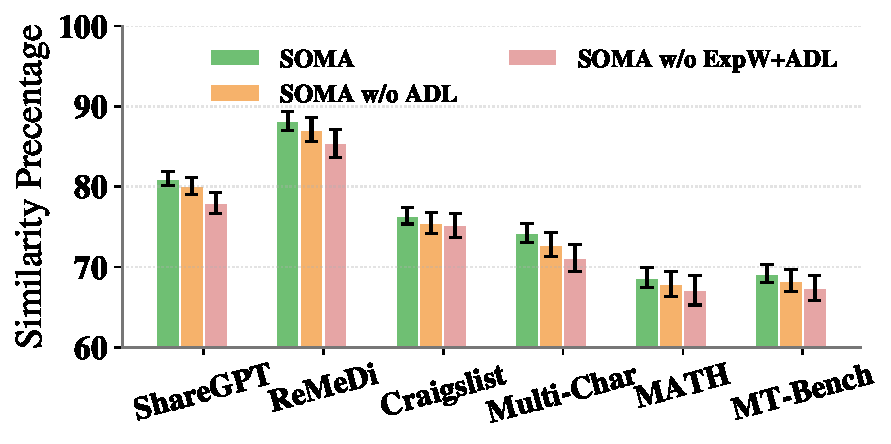
\includegraphics[width=\linewidth]{figure/ablation_qwen.pdf}
    \caption{Qwen ablation.}
    \label{fig:qwen_ablation}
  \end{subfigure}\hfill
  \begin{subfigure}[t]{0.281\textwidth}
    \centering
    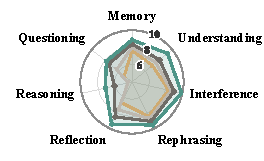
\includegraphics[width=\linewidth]{figure/mt_radar.pdf}
    \caption{Ability profile.}
    \label{fig:mt_radar}
  \end{subfigure}
  \vspace{-2mm}
  \caption{Component and capability analysis. Anti-degeneration regularization and expectation-weighted divergence both improve mining on LLaMA (a) and Qwen (b). (c) MT-Bench-101 ability profile of \textbf{Surrogate}~\textcolor{radarsur}{$\blacktriangle$}, \textbf{History-Prefix}~\textcolor{radarhp}{$\blacktriangledown$}, \textbf{History-FT}~\textcolor{radarft}{$\blacklozenge$}, and \textbf{SOMA}~\textcolor{radarsoma}{$\bullet$}.}
  \label{fig:token_ablation}
\vspace{-3mm}
\end{figure}

\begin{figure}[!t]
  \centering
  \begin{subfigure}[t]{0.525\textwidth}
    \centering
    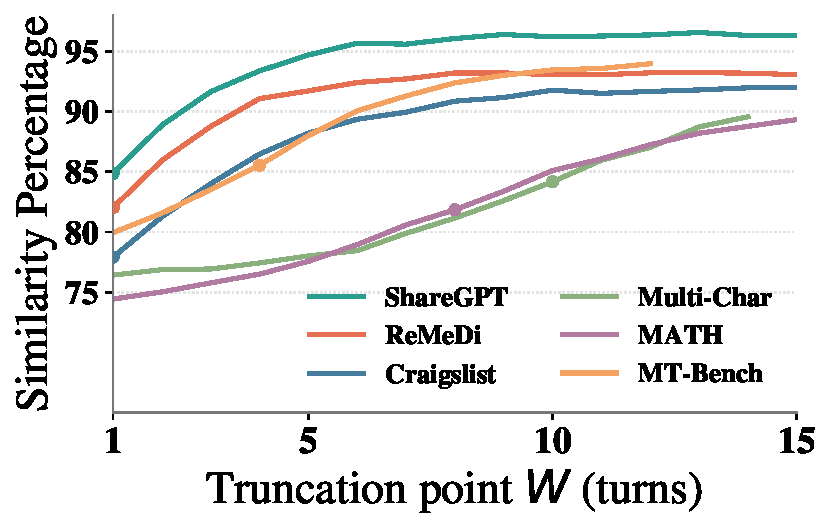
\includegraphics[width=\linewidth]{figure/truncation_trend.pdf}
    \caption{Similarity under different switch points.}
  \end{subfigure}\hfill
  \begin{subfigure}[t]{0.445\textwidth}
    \centering
    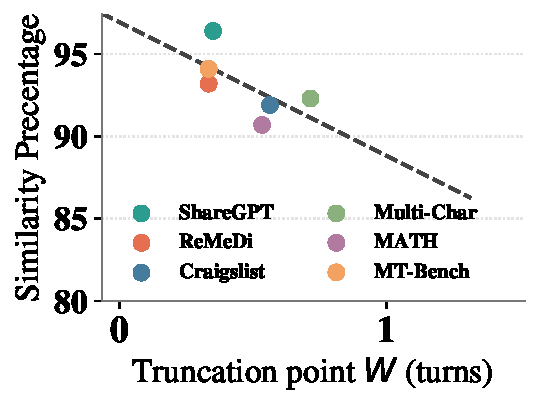
\includegraphics[width=\linewidth]{figure/truncation_vs_similarity.pdf}
    \caption{\rev{Relative switch point} vs.\ final similarity.}
  \end{subfigure}
  \vspace{-2mm}
  \caption{Warm-start and switching behavior. Easier local-dialogue settings switch earlier, while reasoning-heavy or multi-party settings need longer warm starts and achieve lower final similarity.}
  \label{fig:app_switching}
\vspace{-3mm}
\end{figure}

We next test when SOMA's locality assumption holds and how rollback helps when it fails. Figure~\ref{fig:operating}(b) shows that full-history MATH performance stays stable across turn buckets, while no-history performance drops sharply in later turns\rev{, from a 3.1-point EM loss on turns 1--3 to a 21.9-point loss on turns 7 and later}. This means later turns are not simply easier; they remain strongly dependent on the earlier dialogue context. Figure~\ref{fig:operating}(c) then evaluates abrupt topic shifts. Without rollback, similarity drops substantially. With SOMA's drift-aware rollback, \rev{similarity returns to within 2.1--2.6 points of the clean setting (e.g., $88.5\to94.1$ vs.\ $96.4$ on ShareGPT), with 88.9--90.8\% of shifts detected and 3.8--4.3\% false rollbacks.} These results show that SOMA should be viewed as a local serving strategy with automatic fallback. \rev{Figure~\ref{fig:app_switching} shows the warm-start side. Goal-anchored dialogues (ShareGPT, ReMeDi, Craigslist) reach high similarity after a few turns, while reasoning-heavy or multi-party ones (MATH, Multi-Char) need longer warm starts and level off lower. The best switch point thus seems data-dependent, and the gate picks it per session.}


\vspace{-0.2em}
\section{Conclusion}\label{sec:conclusion}
\vspace{-0.2em}
We presented SOMA, an efficient multi-turn LLM serving framework that uses early dialogue turns to adapt a small surrogate to the original model's session-local behavior. SOMA mines informative soft-prompt directions, distills them with lightweight LoRA adaptation, and switches to the surrogate only when semantic alignment is sufficient. Experiments show that SOMA better preserves original-model responses, improves task-grounded quality, and reduces serving cost once warm-start overhead is amortized. These results suggest that session-local surrogate serving is a practical direction for efficient multi-turn LLM deployment \rev{when sessions are long and locally coherent enough to amortize the warm-start cost, as Table~\ref{tab:break-even} quantifies}.

\rev{\textbf{Limitations.} SOMA is bounded by the surrogate's capacity, needs access to the surrogate's embedding layer for mining, and targets locally coherent sessions of at least a few turns; topic drift is handled by rollback rather than prevented (Appendix~\ref{sec:limitations}).}


\bibliographystyle{plain}
\bibliography{ref}

\appendix

\newpage
\section*{Appendix}


\section{Notations}\label{sec:notation}

This section summarizes all notations used throughout this paper. 

% \begin{table}[h]
% \centering
% \small
% \setlength{\tabcolsep}{8pt}
% \begin{tabular}{l l}
% \toprule
% \textbf{Notations} & \textbf{Definitions or Descriptions} \\ 
% \midrule
% % \multicolumn{2}{l}{\textbf{Dialogue / Data}}\\
% $\mathcal{D}_n=\{(q_t,a_t)\}_{t=1}^n$ & Dialogue prefix of $n$ turns (user $q_t$, model $a_t$) \\
% $q_{\le t}$ & Full history up to turn $t$: $\{q_1,a_1,\dots,q_{t-1},a_{t-1},q_t\}$ \\
% $T_0$ & \# initial turns used for mining/adaptation ($\mathcal{W}$) \\
% $\mathcal{B}$ & Replay buffer of $(q_{\le t}, a_t^F)$ pairs \\
% \midrule
% % \multicolumn{2}{l}{\textbf{Models / Spaces}}\\
% $F,\;G$ & Original (large, black-box) and surrogate (small) models \\
% $\mathcal{M}$ & A generic model; $\mathcal{M}(q_{\le t})=a_t$ \\
% $h_t=f_{\mathcal{M}}(q_{\le t})\in\mathbb{R}^d$ & Hidden state at turn $t$ \\
% $\mathcal{H}_k=\{h_1,\dots,h_k\}$ & Hidden states for first $k$ turns \\
% $\mathcal{M}_k^{T},\;\mathcal{M}_k^{S}$ & Teacher / student local response manifolds \\
% $p_F(\cdot\mid q_{\le t}),\;p_G(\cdot\mid q_{\le t};\theta)$ & Next-token distributions (teacher / student) \\
% $a_t^F,\;a_t^G$ & Text responses from $F$ and $G$ at turn $t$ \\
% \midrule
% % \multicolumn{2}{l}{\textbf{Soft Prompts \& LoRA}}\\
% $P\in\mathbb{R}^{L\times d}$ & Soft prompt  \\
% $\{P_j\}_{j=1}^{k}$ & Bank of $k$ mined soft-prompt directions \\
% $\tilde{s}=V(P)$ & Verbalized prompt sent to black-box teacher $F$ \\
% $\Theta_{\text{LoRA}}$ & Trainable LoRA parameters attached to $G$ \\
% $r_{\text{LoRA}}$ & LoRA rank (e.g., $2\!-\!8$) \\
% \midrule
% % \multicolumn{2}{l}{\textbf{Vocab / Embeddings}}\\
% $\mathcal{V}$ & Student tokenizer vocabulary \\
% $E\in\mathbb{R}^{d\times|\mathcal{V}|}$ & Student embedding matrix; $e_v$ is column for token $v$ \\
% $y_t$ & Teacher token at decoding step $t$ \\
% $\mathcal{N}_k(y_t)$ & Semantic neighborhood of $y_t$ (top-$k$ by cosine in $E$) \\
% $\pi_G(\cdot\mid P,q_{\le t})$ & Student token distribution under prompt $P$ \\
% $\bar e_t = E^\top \pi_G(\cdot\mid P,q_{\le t})$ & Student expectation embedding at step $t$ \\
% $\phi(\cdot)$ & Frozen sentence encoder for fast semantic similarity \\
% \midrule
% % \multicolumn{2}{l}{\textbf{Objectives / Scores}}\\
% $D(\cdot\|\cdot)$ & Distributional divergence (e.g., KL) \\
% $\widehat{D}_t$ & Fast semantic switch score at turn $t$ \\
% $\mathcal{L}_{\text{mine}}$ & Mining loss (semantic unlikelihood + weights) \\
% $\mathcal{L}_{\text{KD}}$ & Black-box KD loss for LoRA distillation (NLL on teacher text) \\
% $\mathcal{L}_{\text{sem}}$ & Semantic alignment: $1-\cos(\phi(a_t^F),\phi(a_t^G))$ \\
% $\mathcal{L}_{\text{stab}}$ & Stability: $\mathrm{KL}(p_G^{\text{pre}}\|p_G^{\text{post}})$ \\
% $w_t$ & Expectation-space weight for step $t$ \\
% \midrule
% % \multicolumn{2}{l}{\textbf{Switching / Drift}}\\
% $m$ & Switch window length (consecutive turns) \\
% $\varepsilon,\varepsilon'$ & Switch threshold and watchdog threshold \\
% $\tau_{\text{drift}}$ & Topic-drift threshold (embedding-space) \\
% \midrule
% % \multicolumn{2}{l}{\textbf{Theory / Complexity}}\\
% $\rho$ & Locality radius of admissible context perturbations \\
% $L$ & Lipschitz constant (local smoothness) \\
% $r$ & Effective rank of teacher–student discrepancy \\
% $\{\lambda_i\}$ & Eigenvalues of discrepancy Fisher / spectrum \\
% $N=k\,T_0\,B$ & Sample count in local KD ($B$ teacher samples per direction) \\
% $\sigma^2$ & Noise proxy for black-box KD / estimator \\
% $\mathcal{R}(\Theta)$ & Capacity/regularization term for tuned params \\
% $\gamma(\rho,L)$ & Local smoothness term in error bound \\
% \bottomrule
% \end{tabular}
% \caption{Notations used throughout this paper.}\label{tab:notations}
% % Scalars are lowercase (e.g., $n$), vectors bold lowercase (e.g., $\boldsymbol{\theta}$), matrices bold uppercase (e.g., $\mathbf{W}$), and sets calligraphic (e.g., $\mathcal{D}_n$).
% \end{table}

\begin{table}[h]
\centering
\caption{Notation summary.}
\label{tab:notation}
\setlength{\tabcolsep}{6pt}
\begin{tabular}{@{}ll@{}}
\toprule
Symbol & Meaning \\
\midrule
$\mathcal{D}_k$ & Dialogue prefix $\{(q_t,a_t)\}_{t=1}^k$ \\
$q_{\le t}$ & Full history up to turn $t$ \\
$F,\,G$ & Original (large) model; surrogate (small) model \\
$S_t$ & \rev{Dialogue state $\mathcal D_{t-1}\oplus q_t$ at turn $t$} \\
$\mathcal{Q}_k$ & \rev{Distribution of later dialogue states after $\mathcal{D}_k$ (local region)} \\
$\mathcal{V}$, $E$ & $G$’s vocabulary; embedding matrix $E\in\mathbb{R}^{d\times|\mathcal{V}|}$ \\
$\Pi_t$ & Next-token distribution of $G$ at turn $t$; entry $\Pi_t[v]$ \\
$\mathbf{e}_v$ & Embedding of token $v$ (column of $E$) \\
$\mathbf{P}\in\mathbb{R}^{L\times d}$ & Soft prompt (row-wise prompt tokens in embedding space) \\
$N_k(u)$ & $k$ nearest neighbors of token $u$ by cosine in $E$ \\
$\overline{\mathbf{e}}_{t,i}$ & Expected embedding $\overline{\mathbf{e}}_{t,i}=E^\top \Pi_{t,i}$ at position $i$ \\
$w_{t,i}$ & Expectation-weighted factor for semantic divergence loss \\
$\mathsf{Gap}_G(S)$ & \rev{Response discrepancy $1-\cos(\phi(a^G(S)),\phi(a^F(S)))\in[0,1]$} \\
$r_t$ & \rev{Anchoring score of warm-start turn $t$ (residual mining loss)} \\
$|B|_{\mathrm{eff}}$ & Effective batch size \rev{$|B|/(m+1)$ under $m$-dependence} \\
$\widehat{\mathsf G}_B$ & \rev{Average gap of the adapted surrogate on a held-out acceptance batch} \\
\bottomrule
\end{tabular}
\end{table}

\section{Related Work}\label{sec:related}

\textbf{Efficient LLM for Multi-turn Dialogues.} Recent efforts to improve multi-turn LLM serving efficiency fall into two main paradigms. The first involves \textbf{single-model approaches} that reduce context length or reuse computation. These include \textit{summarization and context compression}~\citep{wang2025recursively, chen2024compress, xiao2024efficient}, \textit{memory augmentation}~\citep{melz2023enhancing, gutierrez2024hipporag}, and \textit{caching and attention reuse}, \rev{such as CachedAttention~\citep{gao2024cost}, prompt caching~\citep{anthropic_prompt_caching_2024}, resource-aware multi-turn scheduling~\citep{jeong2025accelerating}, isolated per-turn KV compression in FlowKV~\citep{liu2025flowkv}, and adaptive prefill sparsification with progressive KV compression in LoopServe~\citep{li2025loopserve}}. While effective in lowering per-turn cost, these methods still rely on repeated large-model inference, which also leads to high API expenses, latency, and GPU demand. Moreover, they may truncate or underutilize dialogue context, harming performance on complex tasks. The second paradigm adopts \textbf{multi-model approach}, using smaller models for simple queries and escalating difficult ones to larger LLMs~\citep{behera2025towards, schick2023toolformer, ding2024hybrid}, typically via model routing~\citep{shnitzer2023large, ong2024routellmlearningroutellms}\rev{, multi-round routing and aggregation learned with reinforcement learning~\citep{zhang2025routerr1},} and distillation~\citep{hinton2015distilling}. However, pre-trained small models often generalize poorly on complex multi-turn dialogues, while switching models adds inefficiency. 

\rev{\textbf{Relation to systems-level serving and test-time adaptation.} Prefix and KV caching (CachedAttention, prompt caching, FlowKV, LoopServe) reduce the prefill cost of re-processing the history on the \emph{same} large model; the per-token decode cost, memory footprint, and API price of that model are unchanged. SOMA is orthogonal: after the switch it removes the large model from the serving path, and the surrogate can itself be served with prefix caching. Our efficiency comparison already serves every method, including Original, through vLLM with automatic prefix caching enabled (Section~\ref{sec:exp}), so the reported token and latency gains are measured on top of KV-cache reuse. Test-time adaptation methods such as Temp-LoRA~\citep{wang2024templora} and StreamAdapter~\citep{muhtar2024streamadapter} adapt a model to its \emph{own} generated or in-context text; History-FT and SOMA instead perform cross-model distillation, adapting the surrogate to the large model's warm-start responses within the session.}
% Furthermore, recent studies show that LLMs overly rely on early conversational turns~\citep{xiao2023efficient, laban2025llms}, making it harder to maintain coherence and reasoning quality in extended dialogues.


\textbf{Local Manifold Approximation.}  
\rev{We use ``local manifold approximation'' in the informal sense of classical local methods such as LLE~\citep{roweis2000nonlinear}, LTSA~\citep{zhang2007linear}, and Laplacian eigenmaps~\citep{belkin2003laplacian}: a dialogue prefix induces a local region of dialogue states, and SOMA approximates the large model only within that region rather than globally. SOMA does not compute intrinsic dimensions, tangent spaces, or geodesics, and it does not match the hidden spaces of the two models. The local view enters the method only through the output-space discrepancy of Problem~\ref{prob:lma}, which compares responses through a shared sentence encoder, and through the locality gate. Its measurable prediction, that warm-start supervision transfers to later turns until the topic shifts, is tested empirically in Section~\ref{sec:exp} and Appendix~\ref{sec:app_switch}.}

\section{Reproducibility}
In this section, we introduce the details of the experiments in this
paper for reproducibility. At the same time, we have uploaded all necessary code to our GitHub repository to reproduce the results presented in this paper: 
\url{https://anonymous.4open.science/r/SOMA-4175}
. All major experiments are encapsulated as shell scripts, which can be conveniently executed. We introduce the details for reproducibility in the subsections below.

\subsection{Real-World Datasets}\label{sec:app_dataset}

In this section, we briefly present the real-world datasets used in this paper, and all these datasets are commonly used datasets in multi-turn conversation tasks. \textit{ShareGPT}~\citep{chen2024sharegpt4v} is a large-scale collection of high-quality image–text conversations and captions. \textit{ReMeDi}~\citep{yan2022remedi} is a multi-domain Chinese medical dialogue corpus of doctor–patient conversations. \textit{Craigslist}~\citep{he2018decoupling} contains multi-turn buyer–seller negotiation chats from Craigslist, enabling study of bargaining strategies and goal-directed dialogue. \textit{Multi-Char}~\citep{agentlans_multi-character_dialogue_2024} provides multi-character conversational scenarios with role specifications to evaluate coordination and role consistency in multi-party dialogue. \textit{MATH}~\citep{hendrycks2021measuring} is a benchmark of competition-style math problems with step-by-step solutions designed to assess mathematical reasoning in language models. \textit{MT-Bench}~\citep{zheng2023judging} is a multi-turn benchmark to assess response quality across diverse tasks. In this study, we filter out the non-context-dependent dialogues in these datasets. 
% All these datasets are implemented based on Torchvision 0.17.1~\cite{torchvision2016}.
% ShareGPT~\citep{chen2024sharegpt4v}, ReMeDi~\citep{yan2022remedi}, Craigslist~\citep{he2018decoupling}, Multi-Char~\citep{agentlans_multi-character_dialogue_2024}, MATH~\citep{hendrycks2021measuring}, and MT-Bench~\citep{zheng2023judging}

\subsection{Implementation of SOMA}\label{sec:app_implementation}

We implement SOMA based on PyTorch with HuggingFace Transformers, serve inference via vLLM with FlashAttention~\citep{shah2024flashattention}, and run on \rev{Nvidia A6000 GPUs}. Soft–prompt tuning optimizes only the prompt tensor $\mathbf{P}\!\in\!\mathbb{R}^{L\times d}$ on the surrogate $G$ using AdamW, cosine decay, gradient clipping, \rev{and a single forward pass per warm-start turn and step}. The objective combines unlikelihood on a semantic neighborhood, an expectation–weighted penalty using the truncated top–$m$ expectation, and a light anti-degeneration entropy term. \rev{The warm-start context--response pairs, weighted by their anchoring scores $r_t$,} are then used to adapt $G$ with LoRA on \rev{attention and MLP} projections (rank $r$), keeping the base weights frozen; \rev{early stopping is triggered when the training loss stops improving, since all warm-start turns are used for adaptation}. At inference, a cosine closeness gate with a lightweight sentence encoder decides a one–time switch to the adapted surrogate. \rev{All hyperparameters below, including $W$, $|B|$, $M$, and $(k,m)$, are set empirically within the listed ranges; the bounds in Section~\ref{sec:theory} describe how the required margins scale but are too loose at these sample sizes to set them directly.} Prompt length $L\!\in\!\{4, 8,16,32,64\}$; learning rate $\eta\!\in\![1\!\times\!10^{-4},\,5\!\times\!10^{-3}]$; AdamW weight decay $\lambda_{\mathrm{wd}}\!\in\![0,\,10^{-2}]$; gradient clip $\in[0.5,\,1.0]$; neighborhood size $k\!\in\!\{20,50,100\}$; expectation truncation $m\!\in\!\{50,100,200\}$; temperature $\tau\!\in\![0.4,\,1.2]$; expectation weight $\lambda\!\in\![0.5,\,2.0]$; anti–degeneration weight $\beta\!\in\![0.02,\,0.15]$; LoRA rank $r\!\in\!\{4, 8,16,32\}$ with scale $\alpha_{\text{lora}}\!\in\!\{4, 8,16,32\}$; LoRA LR $\eta_{\text{lora}}\!\in\![5\!\times\!10^{-5},\,2\!\times\!10^{-3}]$; warm–start window $W\!\in\![3,\,12]$ turns; acceptance batch $|B|\!\in\![6,\,24]$ contexts; parallel candidates $M\!\in\!\{3,4,5\}$; switch threshold $\varepsilon\!\in\![0.05,\,0.12]$ with $m_{\text{cons}}\!\in\!\{2,3\}$. 
% These choices keep computation modest while aligning with the theory–driven bounds used in the paper.


\subsection{Implementation of Baselines}\label{sec:app_baseline}

\textbf{Original}: We query the large model (family-appropriate: LLaMA-3.1-70B or Qwen-3-8B) with the full dialogue history at every turn to get the responses.

\textbf{Surrogate}: We query the small model (LLaMA-2-7B or Qwen-3-0.6B) with the full dialogue history at every turn to get the responses.

\textbf{History-Prefix}: The surrogate receives the entire conversation produced by the Original up to $t{-}1$ and generates $a_t$; no parameter updates are performed. The switching is the same as SOMA.

\textbf{History-FT}: We fine-tune the surrogate on $(S_t, a_t^{F})$ pairs where $S_t$ is the Original’s full context up to $t$ and $a_t^{F}$ is the next reply, using LoRA on attention projections with early stopping; inference then runs the fine-tuned surrogate without the Original. The switching is the same as SOMA.

\textbf{LLMLingua-2}~\citep{pan2024llmlingua}: We compress the Original’s history at each turn with LLMLingua-2 and feed the compressed summary to the surrogate; we follow the authors’ recommended settings.

\textbf{RouteLLM}~\citep{ong2024routellmlearningroutellms}: We adopt the released router to choose between the Original and the surrogate per turn (complex vs.\ simple queries), following the original settings from the paper.

\subsection{Data Filtering}\label{sec:app_filter}

To ensure that SOMA is evaluated on context-dependent dialogues, we prompt multiple strong LLMs, including GPT-OSS, DeepSeek-V3, and Gemma-2-27B, with the classification prompt shown in Figure~\ref{fig:context_filter}, and retain only conversations that all three models recognize as context-dependent. This avoids model-specific biases and yields a high-quality subset of dialogues where later turns meaningfully depend on earlier turns, matching the use cases in this paper.

\begin{figure}[t]
    \centering
    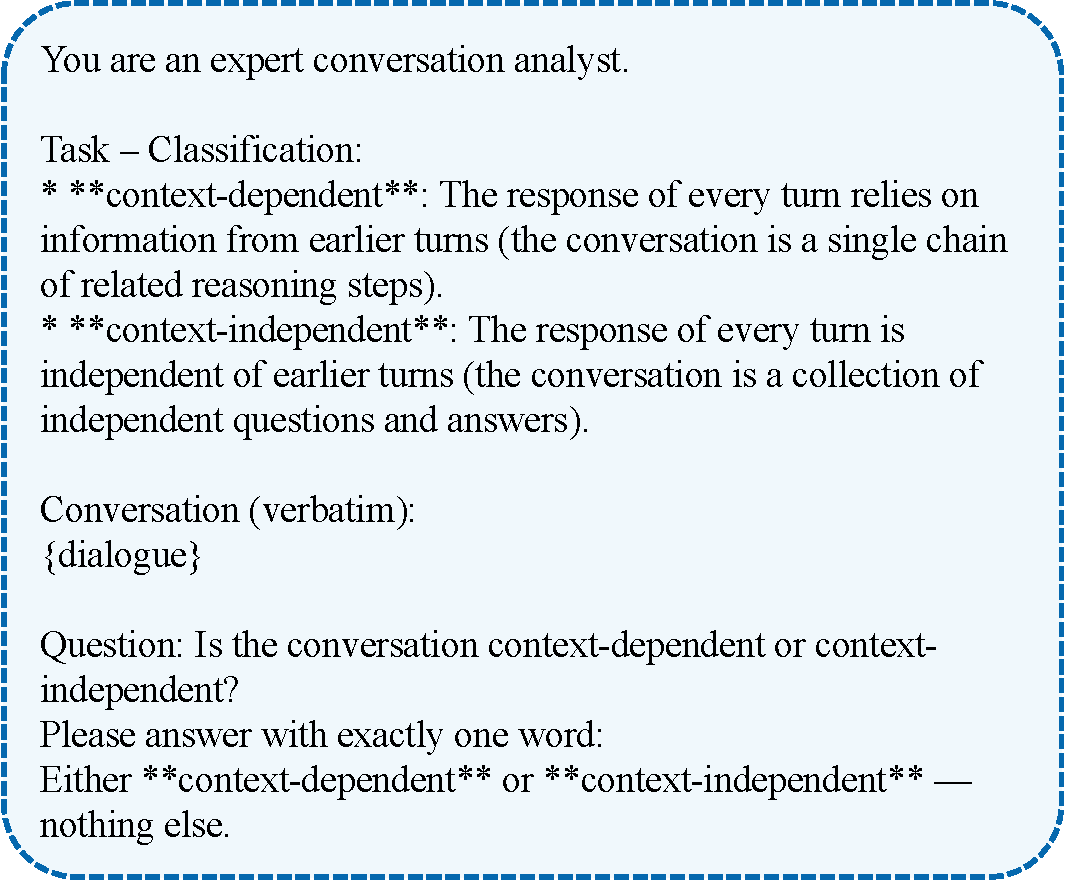
\includegraphics[width=0.8\linewidth]{figure/context_filter.pdf}
    \caption{Instructions for the LLM to filter context-dependent dialogue.}
    \label{fig:context_filter}
\end{figure}

\subsection{Implementation of LLM Judge}\label{sec:app_judge}

The prompt for the LLM judge is shown in Figure~\ref{fig:LLM_judge}. \rev{It adapts the single-answer grading protocol of MT-Bench~\citep{zheng2023judging} and MT-Bench-101~\citep{bai2024mt} to reference-based similarity scoring: the judge receives the original model's response as the reference and scores the surrogate's response on a 0--1 scale along accuracy, reasoning, context integration, and communication. The reference-based framing and the 0--1 scale are our modifications; the MT-Bench protocols grade single answers on a 1--10 scale without a reference. Each response is scored by three judges (GPT-OSS, DeepSeek-V3, and Gemma-2-27B), and we report the mean.}

\begin{figure}[t]
    \centering
    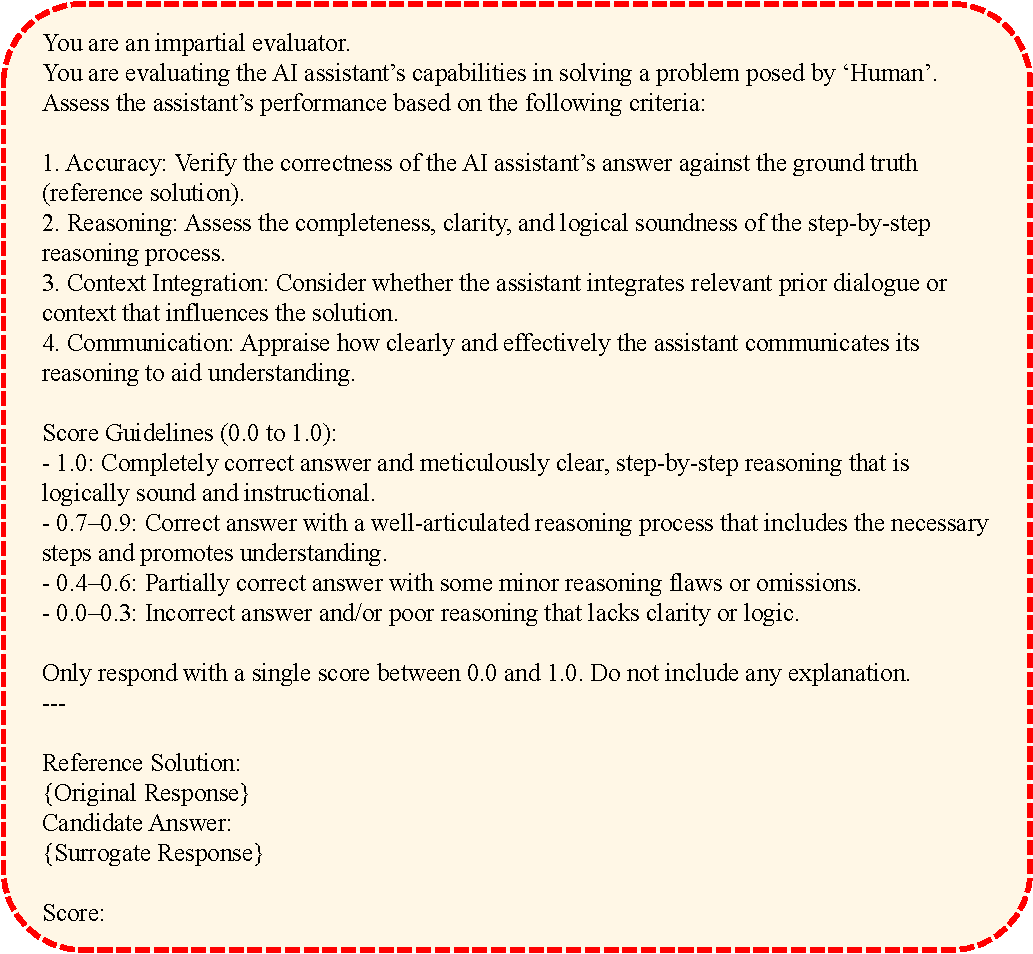
\includegraphics[width=0.8\linewidth]{figure/judge.pdf}
    \caption{Instructions for the LLM judge to evaluate the response similarity.}
    \label{fig:LLM_judge}
\end{figure}

\subsection{Packages Required for Implementation}\label{sec:app_packages}
We perform all experiments on a server equipped with Nvidia A6000 GPUs. Below we list the key packages and their versions used in our implementation:

\begin{itemize}
  \item \textbf{Python} == 3.10
  \item \textbf{pytorch} == 2.8.0 \,+\, CUDA 12.8
  \item \textbf{torchvision} == 0.19.0
  \item \textbf{torchaudio} == 2.8.0
  \item \textbf{numpy} == 1.26.x
  \item \textbf{pandas} == 2.2.x
  \item \textbf{scipy} == 1.12.x
  \item \textbf{cmake} == 3.28+
  \item \textbf{ninja} == 1.11+
  \item \textbf{ipython} == 8.x
  % \item \textbf{jupyter\_core} == 5.x \quad \textbf{jupyter\_client} == 8.x
  \item \textbf{psutil} == 5.9+
  \item \textbf{vllm} == 0.10.2
  \item \textbf{transformers} == 4.56.1
  \item \textbf{accelerate} == 1.9.0
  \item \textbf{bitsandbytes} == 0.46.1
  \item \textbf{sentencepiece} == 0.2.0
  \item \textbf{tiktoken} == 0.11.0
  \item \textbf{einops} == 0.8.1
  \item \textbf{datasets} == 4.0.0
  \item \textbf{huggingface-hub} == 0.34.2
  \item \textbf{safetensors} == 0.5.3
  \item \textbf{ray} == 2.49.1
  \item \textbf{scikit-learn} == 1.7.1
  % \item \textbf{seaborn} == 0.13.2
  \item \textbf{fastapi} == 0.116.2
  \item \textbf{uvicorn} == 0.35.0
\end{itemize}




\section{Mathematical Concepts}\label{sec:app_math}

Here we provide a more comprehensive view of the
relevant concepts that can be helpful to understand the idea of stratification as discussed in the main
body of the paper.

\begin{definition}[Preimage]
Let $f : X \mapsto Y$ be a function from a set $X$ (\emph{domain}) to a set $Y$ (\emph{codomain}). For any subset $N \subseteq Y$, the \emph{preimage} of $N$ under $f$, denoted $f^{-1}(N)$, is defined as:
\[
f^{-1}(N) = \{ x \in X \mid f(x) \in N \}.
\]
\end{definition}
In other words, $f^{-1}(N)$ consists of all elements in the domain $X$ that are mapped into the subset $N$ of the codomain $Y$, regardless of whether every element of $N$ has a preimage.

\begin{definition}[Metric Space]
A set \( X \), whose elements are called points, is said to be a \emph{metric space} if for any two points \( p, q \in X \), there is an associated real number \( d(p, q) \), called the \emph{distance} from \( p \) to \( q \), such that the following three conditions hold:
\begin{enumerate}
    \item \( d(p, q) \geq 0 \), and \( d(p, q) = 0 \iff p = q \);
    \item \( d(p, q) = d(q, p) \) (symmetry);
    \item \( d(p, q) \leq d(p, r) + d(r, q) \) for any \( r \in X \) (triangle inequality).
\end{enumerate}
Any function satisfying these properties is called a \emph{distance function}, or a \emph{metric}.
\end{definition}

\begin{definition}[Neighborhood]
Let \( X \) be a metric space. A set \( N_r(p) \subset X \) is called a \emph{neighborhood} of a point \( p \in X \) if it consists of all points \( q \in X \) such that \( d(p, q) < r \) for some radius \( r > 0 \). The number \( r \) is called the \emph{radius} of the neighborhood.
\end{definition}


\begin{definition}[Continuous]
Let $X$ and $Y$ be two topological spaces. A function $f : X \mapsto Y$ is \emph{continuous} if for each point $x \in X$ and each neighborhood $N$ of $f(x)$ in $Y$, the set $f^{-1}(N)$ is a neighborhood of the point $x \in X$ in the domain.
\end{definition}

\begin{definition}[Topological Equivalence or Homeomorphism]
A function $h : X \mapsto Y$ is called a \emph{homeomorphism} if it is one-to-one, continuous, and has a continuous inverse function. When such a function exists, $X$ and $Y$ are called \emph{homeomorphic} (or \emph{topologically equivalent}) spaces.
\end{definition}

\begin{definition}[Open Set]
A subset \( U \subseteq X \) is called an \emph{open set} if for every point \( p \in U \), there exists a neighborhood \( N_r(p) \subseteq U \). That is, each point in \( U \) has some "wiggle room" around it that still lies entirely within the set \( U \) itself.
\end{definition}

\begin{definition}[Countable Base (Second Countability)]
Let \( X \) be a topological space. A collection \( \mathcal{B} \) of open subsets of \( X \) is called a \emph{base} (or \emph{basis}) for the topology on \( X \) if for every open set \( U \subseteq X \) and every point \( x \in U \), there exists a set \( B \in \mathcal{B} \) such that
\[
x \in B \subseteq U.
\]

If there exists a base \( \mathcal{B} \) that is \emph{countable}, then the space \( X \) is said to be \emph{second countable} or to have a \emph{countable base}; Euclidean spaces, with balls of rational radii around rational points, are a standard example.
\end{definition}

\begin{definition}[Hausdorff Space]
A topological space with the property that two distinct points can always be surrounded by disjoint open sets is called a \emph{Hausdorff space}.
\end{definition}

Essentially, Hausdorff spaces are the spaces where any two points being ``far off'' is defined.

\begin{definition}[Manifold]
A \emph{manifold} of dimension \( n \) is a second-countable Hausdorff topological space in which each point has a neighborhood homeomorphic to Euclidean space \( \mathbb{R}^n \).
\end{definition}

\begin{definition}[Smooth Manifold]
A \emph{smooth manifold} is a manifold \( \mathcal{M} \) equipped with a collection of coordinate charts (i.e., homeomorphisms \( \varphi: U \to \mathbb{R}^n \) for open sets \( U \subseteq \mathcal{M} \)) such that all \emph{transition maps} between overlapping charts,
\[
\varphi_j \circ \varphi_i^{-1} : \varphi_i(U_i \cap U_j) \rightarrow \varphi_j(U_i \cap U_j),
\]
are infinitely differentiable (i.e., \( C^\infty \)). This structure is known as a \emph{smooth atlas}, and it allows calculus to be performed on the manifold.
\end{definition}

\section{Theoretical Results and Proofs}\label{sec:app_proof}

\rev{This appendix states and proves the results used in Section~\ref{sec:theory}. Each statement lists its assumptions, and Section~\ref{sec:warm-start} discusses where our implementation departs from them.

\textbf{Dependence and effective sample size.}
Consecutive dialogue turns are not independent. We assume that the per-turn statistics $Z_1,\ldots,Z_N$ form an $m$-dependent sequence, that is, $\{Z_s\}_{s\le t}$ and $\{Z_s\}_{s>t+m}$ are independent for every $t$, and we define the effective sample size $N_{\mathrm{eff}}=N/(m+1)$; independent samples correspond to $m=0$. For such sequences Hoeffding's inequality holds with $N$ replaced by $N_{\mathrm{eff}}$: if each $Z_s$ takes values in an interval of length $R$, then for every $u>0$
\[
\Pr\Big(\frac1N\sum_{s=1}^{N}\big(Z_s-\mathbb E Z_s\big)\ge u\Big)\le\exp\Big(-\frac{2N_{\mathrm{eff}}\,u^2}{R^2}\Big),
\]
and the same bound holds for the lower tail. This follows from Janson's inequality for sums of partly dependent variables~\citep{janson2004large}, applied to the dependency graph of the sequence, whose fractional chromatic number is at most $m+1$.

\textbf{Locality premise.}
The results below compare statistics measured on warm-start turns with their expectations over the later turns of the session. We therefore assume, as in Section~\ref{sec:prelim}, that warm-start states and later states share the marginal distribution $\mathcal Q_k$. This is the premise that the locality gate monitors and that Figures~\ref{fig:operating}(c) and~\ref{fig:app_switching} test; otherwise they describe only the warm-start distribution.

\bigskip
\textbf{Switching Criterion: Warm-Start Concentration and Acceptance}

\begin{lemma}[Warm-Start Concentration]\label{lem:warmstart}
Let $h(S)\in[0,1]$ be a local statistic that is fixed before the window is observed, such as $\mathsf{Gap}_{\Theta}(S)$ for a fixed adapter $\Theta$ or the distance of a query to a fixed centroid. Let $h(S_1),\ldots,h(S_W)$ be $m$-dependent with common mean $h^\star=\mathbb E_{S\sim\mathcal Q_k}[h(S)]$, and write $\hat h_W=\frac1W\sum_{t=1}^{W}h(S_t)$. Then, with probability at least $1-\delta$,
\[
\big|\hat h_W-h^\star\big|\le\eta_W(\delta):=\sqrt{\frac{\log(2/\delta)}{2W_{\mathrm{eff}}}} .
\]
\end{lemma}

\paragraph{Proof of Lemma~\ref{lem:warmstart}.}
Apply the $m$-dependent Hoeffding inequality with $R=1$ to each tail at level $\delta/2$. Setting $\exp(-2W_{\mathrm{eff}}u^2)=\delta/2$ gives $u=\eta_W(\delta)$, and a union bound over the two tails gives the claim.
\hfill$\square$

\paragraph{Statement: Proposition~\ref{thm:detection}.}
Let the adapter $\Theta$ be fixed given the adaptation data, and let the acceptance batch $B=\{S_1,\ldots,S_{|B|}\}$ be disjoint from that data and drawn from $\mathcal Q_k$ as an $m$-dependent sequence. Let $\widehat{\mathsf G}_B=\frac1{|B|}\sum_{j}\mathsf{Gap}_{\Theta}(S_j)$ and $\mathsf G^\star=\mathbb E_{S\sim\mathcal Q_k}[\mathsf{Gap}_{\Theta}(S)]$. Then, with probability at least $1-\delta$,
\[
\mathsf G^\star\le\widehat{\mathsf G}_B+\gamma_B(\delta),\qquad \gamma_B(\delta)=\sqrt{\frac{\log(1/\delta)}{2|B|_{\mathrm{eff}}}} .
\]
In particular, if $\widehat{\mathsf G}_B\le\varepsilon-\gamma_B(\delta)$, then $\mathsf G^\star\le\varepsilon$ with probability at least $1-\delta$.

\paragraph{Proof of Proposition~\ref{thm:detection}.}
Condition on the adaptation data. Because $B$ is disjoint from it, $\Theta$ is fixed, and $\mathsf{Gap}_{\Theta}(S_1),\ldots,\mathsf{Gap}_{\Theta}(S_{|B|})$ are $m$-dependent with mean $\mathsf G^\star$ and range $R=1$. The lower-tail inequality gives $\Pr(\widehat{\mathsf G}_B-\mathsf G^\star\le-u)\le\exp(-2|B|_{\mathrm{eff}}u^2)$, and setting the right-hand side to $\delta$ gives $u=\gamma_B(\delta)$. On the complementary event, $\mathsf G^\star<\widehat{\mathsf G}_B+\gamma_B(\delta)\le\varepsilon$ if $\widehat{\mathsf G}_B\le\varepsilon-\gamma_B(\delta)$.
\hfill$\square$

\textbf{When the acceptance batch is reused.}
If $B$ overlaps the adaptation data, $\Theta$ depends on the $S_j$ in $B$. The gaps then no longer have mean $\mathsf G^\star$ given $\Theta$, $\widehat{\mathsf G}_B$ is biased downward by the fit, and Proposition~\ref{thm:detection} does not apply. Our implementation reuses the warm-start turns in this way (Appendix~\ref{sec:app_rationale}); holding out part of the warm-start window would restore the bound at the cost of fewer adaptation examples. The bound is also loose at the sample sizes used here: for $\delta=0.05$, $m=0$, and $|B|=24$, $\gamma_B=0.25$, which already exceeds the thresholds $\varepsilon\in[0.05,0.12]$. It therefore describes how the required margin scales with $|B|_{\mathrm{eff}}$ rather than setting the thresholds.

\begin{corollary}[Switching Rule]\label{cor:switch}
Let the locality statistic $h$ satisfy the conditions of Lemma~\ref{lem:warmstart}, and let $B$ satisfy those of Proposition~\ref{thm:detection}. If $\widehat{\mathsf G}_B\le\varepsilon-\gamma_B(\delta)$ and $\hat h_W\le\tau-\eta_W(\delta)$, then, with probability at least $1-2\delta$, both $\mathsf G^\star\le\varepsilon$ and $h^\star\le\tau$.
\end{corollary}

\paragraph{Proof of Corollary~\ref{cor:switch}.}
By Lemma~\ref{lem:warmstart}, $h^\star\le\hat h_W+\eta_W(\delta)\le\tau$ with probability at least $1-\delta$. By Proposition~\ref{thm:detection}, $\mathsf G^\star\le\varepsilon$ with probability at least $1-\delta$. A union bound shows that both hold with probability at least $1-2\delta$.
\hfill$\square$

\bigskip
\textbf{Coverage and Suboptimality to Determine the Number of Soft-Prompt Candidates}

Assume that the mining objective is locally quadratic with curvature $\mathbf H_T\succeq 0$ whose top eigenvector $\boldsymbol v_1$ lies in an $r_{\mathrm{act}}$-dimensional active subspace. SOMA draws its $M$ candidate prompts from an isotropic Gaussian, so their projections onto this subspace point in independent, uniformly random directions. The results below bound the probability that one of them starts within angle $\theta$ of $\boldsymbol v_1$, and the fraction of the top curvature that such a direction retains. They concern the initial directions rather than the optimized prompts, and we set $M\in\{3,4,5\}$ empirically (Appendix~\ref{sec:app_implementation}).

\begin{proposition}[Coverage of the Best Local Direction]\label{thm:coverage}
Let $r_{\mathrm{act}}\ge 2$, let $\boldsymbol v_1$ be a unit vector in an $r_{\mathrm{act}}$-dimensional subspace, and draw $\boldsymbol u_1,\ldots,\boldsymbol u_M$ i.i.d.\ from $\mathrm{Unif}(\mathbb S^{r_{\mathrm{act}}-1})$ in that subspace. For $\theta\in(0,\pi/2]$, let
\[
p_{r_{\mathrm{act}}}(\theta)=\Pr\big(\angle(\boldsymbol u_1,\boldsymbol v_1)\le\theta\big)=\tfrac12\,I_{\sin^2\theta}\Big(\tfrac{r_{\mathrm{act}}-1}{2},\tfrac12\Big),
\]
where $I_x(\cdot,\cdot)$ is the regularized incomplete beta function. Then
\[
\Pr\Big(\min_{m\le M}\angle(\boldsymbol u_m,\boldsymbol v_1)\le\theta\Big)=1-\big(1-p_{r_{\mathrm{act}}}(\theta)\big)^M,
\qquad
p_{r_{\mathrm{act}}}(\theta)\ge\frac{(\sin\theta)^{r_{\mathrm{act}}-1}}{(r_{\mathrm{act}}-1)\,\mathrm B\big(\frac{r_{\mathrm{act}}-1}{2},\frac12\big)} .
\]
For example, $p_{r_{\mathrm{act}}}(\pi/2)=1/2$ for every $r_{\mathrm{act}}$. Isotropic Gaussian initializations satisfy the sampling assumption, because the normalized projection of $\mathcal N(\boldsymbol 0,\sigma^2\mathbf I)$ onto a fixed subspace is uniformly distributed on the unit sphere of that subspace.
\end{proposition}

\paragraph{Proof of Proposition~\ref{thm:coverage}.}
\textbf{Step 1: Exact cap probability.}
Write $r=r_{\mathrm{act}}$ and $T=\langle\boldsymbol u_1,\boldsymbol v_1\rangle$. For $\boldsymbol u_1$ uniform on $\mathbb S^{r-1}$, $T$ is symmetric about $0$ and $T^2\sim\mathrm{Beta}(\frac12,\frac{r-1}{2})$, so $1-T^2\sim\mathrm{Beta}(\frac{r-1}{2},\frac12)$. For $\theta\le\pi/2$ we have $\cos\theta\ge0$, hence
\[
\Pr(T\ge\cos\theta)=\tfrac12\Pr(T^2\ge\cos^2\theta)=\tfrac12\Pr(1-T^2\le\sin^2\theta)=\tfrac12\,I_{\sin^2\theta}\big(\tfrac{r-1}{2},\tfrac12\big).
\]

\textbf{Step 2: Lower bound.}
Let $a=(r-1)/2$ and $x=\sin^2\theta$. Since $(1-s)^{-1/2}\ge1$ on $[0,1)$,
\[
I_x\big(a,\tfrac12\big)=\frac{1}{\mathrm B(a,\frac12)}\int_0^x s^{a-1}(1-s)^{-1/2}\,\mathrm ds\;\ge\;\frac{1}{\mathrm B(a,\frac12)}\int_0^x s^{a-1}\,\mathrm ds=\frac{x^{a}}{a\,\mathrm B(a,\frac12)},
\]
so $p_r(\theta)\ge x^{a}/\big(2a\,\mathrm B(a,\frac12)\big)=(\sin\theta)^{r-1}/\big((r-1)\,\mathrm B(\frac{r-1}{2},\frac12)\big)$.

\textbf{Step 3: Independence across $M$ samples.}
The $M$ draws are independent, so none of them falls in the cap with probability $(1-p_r(\theta))^M$, which gives the coverage probability.
\hfill$\square$

\bigskip
\begin{lemma}[Directional Suboptimality]\label{lem:subopt}
Let $\mathbf H_T\succeq 0$ have largest eigenvalue $\lambda_1$ and top eigenvector $\boldsymbol v_1$. For any unit $\boldsymbol{\hat u}$ with $\angle(\boldsymbol{\hat u},\boldsymbol v_1)\le\theta\le\pi/2$,
\[
\boldsymbol{\hat u}^{\!\top}\mathbf{H}_T\boldsymbol{\hat u} \;\ge\; \lambda_1 \cos^2\!\theta,
\qquad
\lambda_1 - \boldsymbol{\hat u}^{\!\top}\mathbf{H}_T\boldsymbol{\hat u} \;\le\; \lambda_1 \sin^2\!\theta.
\]
\end{lemma}

\paragraph{Proof of Lemma~\ref{lem:subopt}.}
Let $\varphi=\angle(\boldsymbol{\hat u},\boldsymbol v_1)\le\theta$ and decompose $\boldsymbol{\hat u}=\cos\varphi\,\boldsymbol{v}_1+\sin\varphi\,\boldsymbol{w}$ with $\|\boldsymbol{w}\|_2=1$ and $\boldsymbol{w}\perp\boldsymbol{v}_1$. Because $\mathbf H_T\boldsymbol v_1=\lambda_1\boldsymbol v_1$, the cross term vanishes, and
\[
\boldsymbol{\hat u}^{\!\top}\mathbf{H}_T\boldsymbol{\hat u}
=
\lambda_1\cos^2\!\varphi
+
\sin^2\!\varphi\sum_{j\ge 2}\lambda_j \langle \boldsymbol{v}_j,\boldsymbol{w}\rangle^2
\;\ge\;
\lambda_1\cos^2\!\varphi\;\ge\;\lambda_1\cos^2\!\theta,
\]
since $\lambda_j\ge 0$ and $\cos^2$ is decreasing on $[0,\pi/2]$. Subtracting from $\lambda_1$ gives the residual bound.
\hfill$\square$

\bigskip
\begin{corollary}[Candidate Budget]\label{col:M}
Under the conditions of Proposition~\ref{thm:coverage}, the coverage probability within angle $\theta$ is at least $1-\delta$ whenever $M\ge\log(1/\delta)\big/\log\big(1/(1-p_{r_{\mathrm{act}}}(\theta))\big)$. Because $\log(1/(1-p))\ge p$, the simpler condition $M\ge(r_{\mathrm{act}}-1)\,\mathrm B\big(\frac{r_{\mathrm{act}}-1}{2},\frac12\big)\log(1/\delta)/(\sin\theta)^{r_{\mathrm{act}}-1}$ also suffices. Together with Lemma~\ref{lem:subopt}, this trades candidate count against the quality of the best direction.
\end{corollary}

\paragraph{Proof of Corollary~\ref{col:M}.}
Coverage fails with probability $(1-p)^M$, where $p=p_{r_{\mathrm{act}}}(\theta)$, and $(1-p)^M\le\delta$ holds if and only if $M\log(1/(1-p))\ge\log(1/\delta)$. The second condition follows from $\log(1/(1-p))\ge p$ and the lower bound on $p$ in Proposition~\ref{thm:coverage}.
\hfill$\square$}


\section{Additional Experimental Results}
\label{sec:app_exp}

This appendix provides supporting results that complement the main experiments: dataset-level token costs, the effect of warm-start length on switching, and the empirical variance concentration behind the switching bound in Section~\ref{sec:warm-start}.

\subsection{Additional Efficiency Results}
\label{sec:app_eff}

The main text reports the amortized break-even analysis and throughput. Here we provide the dataset-level token results for both model families. Figure~\ref{fig:app_token_costs} shows that \rev{SOMA uses the fewest tokens per dialogue on 11 of the 12 dataset--family pairs; the exception is Craigslist with LLaMA, where Original uses 3\% fewer}. The reason is that after switching, SOMA serves later turns with the adapted surrogate and a compressed context rather than repeatedly sending the full growing history. This avoids the large token cost of Original and History-Prefix while retaining stronger response similarity than directly using the unadapted surrogate.

\begin{figure}[t]
  \centering
  \begin{minipage}[t]{0.49\textwidth}
    \centering
    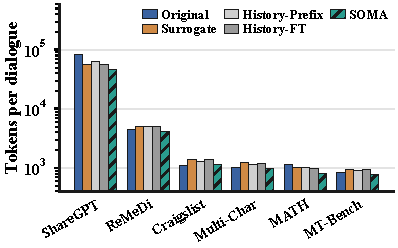
\includegraphics[width=\linewidth]{figure/llama_token_costs.pdf}
    \vspace{-2mm}
    \centerline{\small (a) LLaMA family}
  \end{minipage}\hfill
  \begin{minipage}[t]{0.49\textwidth}
    \centering
    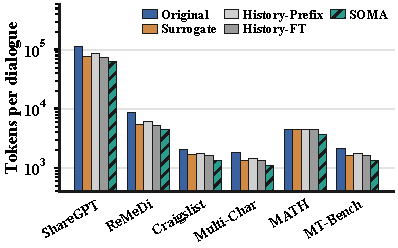
\includegraphics[width=\linewidth]{figure/qwen_token_costs.pdf}
    \vspace{-2mm}
    \centerline{\small (b) Qwen family}
  \end{minipage}
  \vspace{-1mm}
  \caption{Average tokens per dialogue across six datasets. SOMA reduces token usage by avoiding repeated full-history serving after switching.}
  \label{fig:app_token_costs}
\end{figure}

\subsection{Warm-Start Length and Switching Behavior}
\label{sec:app_switch}

The main text (Figure~\ref{fig:app_switching}) reports how final similarity depends on the switch point. The sweep uses warm-start windows \(W\in[1,15]\) and measures the final response similarity after switching. Once the curve flattens, adding more warm-start turns brings little quality gain but delays the efficiency benefit, so short warm starts suffice for general or goal-anchored chats, while compositional reasoning and multi-party dialogues need more evidence before switching.

\subsection{Empirical Variance Concentration}
\label{sec:app_variance}

Finally, we examine how the variance of surrogate--teacher similarity changes with the warm-start window \(W\). For each dataset, we compute the empirical standard deviation across dialogues at each truncation point. Figure~\ref{fig:variance} shows that variance decreases as \(W\) grows: early turns are highly variable, while larger warm-start windows enter a more stable regime. This trend is consistent with the concentration behavior used in Lemma~\ref{lem:warmstart} and the switching bound in \rev{Proposition}~\ref{thm:detection}. In other words, early turns provide the largest information gain, while later warm-start turns mainly reduce uncertainty until the switching decision becomes stable.

\begin{figure}[t]
  \centering
  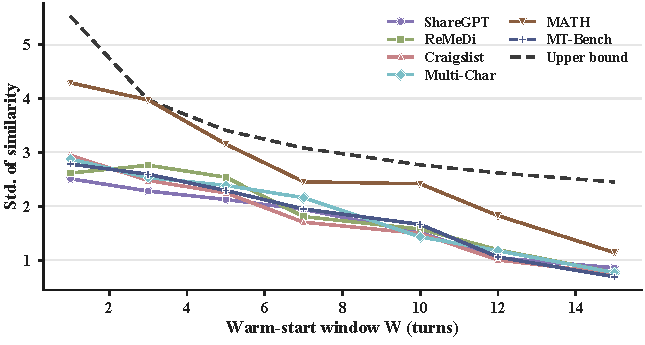
\includegraphics[width=0.78\textwidth]{figure/variance_vs_W.pdf}
  \caption{Variance of response similarity versus warm-start window \(W\). Larger warm-start windows reduce variance and support more stable switching decisions.}
  \label{fig:variance}
\end{figure}


\section{Design Rationale and Serving Considerations}
\label{sec:app_rationale}
\rev{This section collects design questions raised in review that the main text only touches on.

\textbf{Choice of soft prompts and of an adversarial objective.}
Soft prompts are a convenient probe for three practical reasons: they are differentiable, so a handful of gradient steps on the surrogate $G$ can search a continuous neighborhood of the warm-start context instead of enumerating discrete paraphrases; they live in $G$'s own embedding space, so the semantic neighborhood $\mathcal N_k(\cdot)$ and the expected-embedding weight are computed with the same token embeddings and reuse the logits of a single forward pass; and the ANN-based neighborhood keeps the per-step cost proportional to $k+m$ rather than $|\mathcal V|$. Alternative perturbations (input noise, paraphrasing, or adversarial token substitution) can also explore beyond the finite warm-start turns, but they either require an external paraphraser or a discrete search, and they do not directly expose which \emph{directions} in $G$'s input space make $G$ diverge from $F$. We push $G$ away from $F$ rather than toward it because the score must measure how robust the agreement is, not how much agreement a prompt can add. A constructive (divergence-minimizing) prompt would raise the agreement on every turn and yield a signal confounded with the capacity of the prompt itself; an adversarial prompt removes the agreement that is easy to remove, and $r_t$ records what survives. The prompts are then discarded, and only the anchoring scores $r_t$ enter the LoRA objective in Eq.~\ref{eq:lora-ft} as per-turn training weights.

\textbf{Relation to divergence-weighted History-FT and Random-FT.}
The LoRA objective in Eq.~\ref{eq:lora-ft} weights every warm-start turn by its anchoring score $\omega_t\propto r_t$, so SOMA can be read as a weighted History-FT whose weights come from prompt probing rather than from the raw output divergence between $G$ and $F$ on the warm-start turn. The two weightings measure different things and point in opposite directions: raw output divergence emphasizes turns that the \emph{unperturbed} surrogate currently gets wrong, whereas the anchoring score emphasizes turns whose teacher response the surrogate still predicts \emph{after} an adversarial perturbation, i.e., responses that are determined by the dialogue state and hence likely to transfer to later turns. The ablation in Figure~\ref{fig:llama_ablation} isolates the contributions of the mining objective's two terms, but it does not include a baseline that weights History-FT by raw output divergence or one that samples training turns uniformly at random with the same LoRA budget; we consider both key controls and leave them, with a prompt-length sweep, to future work.

\textbf{Robustness, divergence, and the perturbation space.}
We do not prove that robustness under prompt perturbations is a better predictor of adaptation utility than direct output divergence, nor that the continuous perturbation space of $\mathbf P$ covers the space of natural-language future turns. We therefore treat these as modeling assumptions and test them indirectly: the topic-shift stress test (Figure~\ref{fig:operating}(c)) probes future turns that leave the mined region, and the warm-start sweep (Appendix~\ref{sec:app_switch}) shows how much of the local behavior is captured as the window grows. A direct empirical comparison of the two weightings is the most informative next step for validating the mining objective.

\textbf{Number of large-model calls and target consistency.}
The original model $F$ is queried once per warm-start turn to serve the user; these $W$ responses are stored and reused as the mining targets $a_t^F$, as the LoRA targets, and as the references for the acceptance gate. $F$ is not re-queried while $\mathbf P$ is optimized, so the targets are never stale with respect to the dialogue state, and the soft prompt perturbs only the surrogate side of the objective. Because the acceptance gate reuses these turns, the acceptance bound of Section~\ref{sec:warm-start} does not certify the gate as implemented; holding out part of the warm-start window would restore it at the cost of fewer adaptation examples. Prompt mining and LoRA adaptation run entirely on the surrogate and consist of a small number of forward--backward passes over the $W$ warm-start turns ($M$ candidate prompts times the mining iterations, followed by the LoRA steps). Their wall-clock cost is part of the end-to-end latency reported in Figure~\ref{fig:operating}(a).

\textbf{Drift detection.}
The drift statistic is the cosine distance between recent queries and the warm-start centroid, monitored over a sliding window; rollback triggers after $m_{\mathrm{cons}}$ consecutive violations. Because the statistic is continuous, gradual drift raises it progressively rather than only at abrupt shifts, and Corollary~\ref{cor:switch} would bound the probability of accepting a surrogate whose true gap exceeds the margin if the acceptance batch were held out and the centroid fixed in advance. As implemented, both come from the warm-start turns, so the initial switch is a heuristic check (Section~\ref{sec:warm-start}). Re-switching after a rollback differs: its acceptance batch and refreshed centroid come from the turns $F$ serves after the shift, which the adapter never saw, so the held-out condition of Proposition~\ref{thm:detection} holds for that decision. The gate does not certify that the centroid distance tracks every form of quality degradation, which is why we also report the false-rollback and detection rates in Figure~\ref{fig:operating}(c).

\textbf{Serving many session-local adapters.}
A LoRA adapter of rank $r$ on the attention and MLP projections of LLaMA-2-7B has about $2.5r$ million parameters ($\approx 20$M parameters, or roughly 40~MB in bfloat16, for $r=8$), i.e., well under $1\%$ of the surrogate. Multi-adapter serving systems batch requests from many adapters over a single copy of the base weights and page adapters between host and GPU memory~\citep{sheng2023slora}, so GPU residency is bounded by the number of concurrently \emph{switched} sessions rather than by the total number of sessions, and an adapter is discarded as soon as its session ends. The mining and adaptation steps for a session are independent of other sessions and can be scheduled as short background jobs on the surrogate replica. We did not benchmark multi-node concurrent adapter scheduling; the reported latencies are for the single-session serving path described in Section~\ref{sec:method}.}

\section{Broader Impact}
\label{sec:broader_impact}

SOMA aims to reduce the cost and latency of multi-turn LLM serving by replacing repeated large-model inference with session-local surrogate serving. This can make interactive LLM systems more efficient, accessible, and environmentally sustainable. At the same time, using a smaller surrogate may introduce quality degradation if the dialogue leaves the learned local state, especially in high-stakes settings such as medical, legal, or financial assistance. SOMA mitigates this risk through semantic acceptance and drift-aware rollback, but deployment should still include monitoring, conservative thresholds, and human oversight where errors may cause harm. Since SOMA uses dialogue history for local adaptation, practical deployments should also apply data minimization, retention limits, and privacy-preserving processing of the dialogue history.



\section{Limitations and Future Work}
\label{sec:limitations}

SOMA has several limitations. First, the surrogate's capacity limits how closely it can match the original model. When the small--large model gap is very large, some behaviors cannot be recovered by session-local adaptation alone. Second, soft-prompt mining requires access to the surrogate tokenizer and embedding space, which makes SOMA harder to deploy in strict black-box API settings. Third, SOMA is designed for locally coherent dialogues. Abrupt topic changes, noisy warm-start windows, or strong paraphrase shifts can weaken the learned local directions, although the drift gate is designed to reduce persistent degradation. Finally, SOMA introduces a one-time warm-start cost, so it is most suitable for medium-to-long sessions where post-switch savings can amortize the initial adaptation overhead. \rev{Two further limitations concern evaluation. Gradual topic drift is detected by the same continuous centroid statistic as abrupt shifts, but we have only stress-tested abrupt shifts (Figure~\ref{fig:operating}(c)); quality may degrade before the rollback margin is exhausted. We also have not compared SOMA against a History-FT variant weighted by raw output divergence or against uniformly sampled local turns under the same LoRA budget (Appendix~\ref{sec:app_rationale}), so the incremental value of prompt mining over simpler weightings is supported by the component ablation rather than by a direct head-to-head comparison against these alternatives.}

Future work can improve SOMA along several directions. Better drift detectors could make rollback more reliable under topic shifts. Approximate mining methods could reduce the need for internal surrogate access. Multi-region adaptation could support conversations with multiple topics, and privacy-preserving mining could make the method safer for sensitive dialogue settings. Another promising direction is to amortize soft-prompt search across related sessions and extend SOMA to multimodal serving, where early turns often carry images or documents.

% \newpage
\section*{NeurIPS Paper Checklist}

% %%% BEGIN INSTRUCTIONS %%%
% The checklist is designed to encourage best practices for responsible machine learning research, addressing issues of reproducibility, transparency, research ethics, and societal impact. Do not remove the checklist: {\bf The papers not including the checklist will be desk rejected.} The checklist should follow the references and follow the (optional) supplemental material.  The checklist does NOT count towards the page
% limit. 

% Please read the checklist guidelines carefully for information on how to answer these questions. For each question in the checklist:
% \begin{itemize}
%     \item You should answer \answerYes{}, \answerNo{}, or \answerNA{}.
%     \item \answerNA{} means either that the question is Not Applicable for that particular paper or the relevant information is Not Available.
%     \item Please provide a short (1--2 sentence) justification right after your answer (even for \answerNA). 
%    % \item {\bf The papers not including the checklist will be desk rejected.}
% \end{itemize}

% {\bf The checklist answers are an integral part of your paper submission.} They are visible to the reviewers, area chairs, senior area chairs, and ethics reviewers. You will also be asked to include it (after eventual revisions) with the final version of your paper, and its final version will be published with the paper.

% The reviewers of your paper will be asked to use the checklist as one of the factors in their evaluation. While \answerYes{} is generally preferable to \answerNo{}, it is perfectly acceptable to answer \answerNo{} provided a proper justification is given (e.g., error bars are not reported because it would be too computationally expensive'' or ``we were unable to find the license for the dataset we used''). In general, answering \answerNo{} or \answerNA{} is not grounds for rejection. While the questions are phrased in a binary way, we acknowledge that the true answer is often more nuanced, so please just use your best judgment and write a justification to elaborate. All supporting evidence can appear either in the main paper or the supplemental material, provided in appendix. If you answer \answerYes{} to a question, in the justification please point to the section(s) where related material for the question can be found.

% IMPORTANT, please:
% \begin{itemize}
%     \item {\bf Delete this instruction block, but keep the section heading ``NeurIPS Paper Checklist"},
%     \item  {\bf Keep the checklist subsection headings, questions/answers and guidelines below.}
%     \item {\bf Do not modify the questions and only use the provided macros for your answers}.
% \end{itemize} 

%%% END INSTRUCTIONS %%%


\begin{enumerate}

\item {\bf Claims}
    \item[] Question: Do the main claims made in the abstract and introduction accurately reflect the paper's contributions and scope?
    \item[] Answer: \answerYes{}
    \item[] Justification: The abstract and introduction state the main contributions, assumptions, and intended scope of SOMA, and the claims are supported by the method, theory, and experiments.

\item {\bf Limitations}
    \item[] Question: Does the paper discuss the limitations of the work performed by the authors?
    \item[] Answer: \answerYes{}
    \item[] Justification: The paper discusses limitations related to surrogate capacity, session-local assumptions, topic shifts, warm-start overhead, and deployment considerations.

\item {\bf Theory assumptions and proofs}
    \item[] Question: For each theoretical result, does the paper provide the full set of assumptions and a complete (and correct) proof?
    \item[] Answer: \answerYes{}
    \item[] Justification: The theoretical results state the main assumptions and are supported by proof sketches in the main text and detailed arguments in the appendix.

\item {\bf Experimental result reproducibility}
    \item[] Question: Does the paper fully disclose all the information needed to reproduce the main experimental results of the paper to the extent that it affects the main claims and/or conclusions of the paper?
    \item[] Answer: \answerYes{}
    \item[] Justification: The experimental setup, datasets, models, baselines, metrics, and implementation details are described in the paper and appendix, with additional details provided in the anonymized code repository.

\item {\bf Open access to data and code}
    \item[] Question: Does the paper provide open access to the data and code, with sufficient instructions to faithfully reproduce the main experimental results, as described in supplemental material?
    \item[] Answer: \answerYes{}
    \item[] Justification: An anonymized code repository is provided with implementation details, scripts, and instructions for reproducing the main experiments. The experiments use publicly available datasets and models.

\item {\bf Experimental setting/details}
    \item[] Question: Does the paper specify all the training and test details necessary to understand the results?
    \item[] Answer: \answerYes{}
    \item[] Justification: The paper reports the datasets, model families, baselines, metrics, evaluation protocol, and key hyperparameters, with additional configuration details in the appendix and anonymized repository.

\item {\bf Experiment statistical significance}
    \item[] Question: Does the paper report error bars suitably and correctly defined or other appropriate information about the statistical significance of the experiments?
    \item[] Answer: \answerYes{}
    \item[] Justification: The main quantitative tables report mean performance with standard deviations, and the corresponding evaluation protocol is described with the experimental setup.

\item {\bf Experiments compute resources}
    \item[] Question: For each experiment, does the paper provide sufficient information on the computer resources needed to reproduce the experiments?
    \item[] Answer: \answerYes{}
    \item[] Justification: The implementation appendix and anonymized repository provide the relevant compute and runtime details needed to reproduce the reported experiments.

\item {\bf Code of ethics}
    \item[] Question: Does the research conducted in the paper conform, in every respect, with the NeurIPS Code of Ethics?
    \item[] Answer: \answerYes{}
    \item[] Justification: The work uses public datasets and models, does not introduce human-subject data collection, and discusses relevant deployment risks and safeguards.

\item {\bf Broader impacts}
    \item[] Question: Does the paper discuss both potential positive societal impacts and negative societal impacts of the work performed?
    \item[] Answer: \answerYes{}
    \item[] Justification: The paper includes a broader impact discussion covering efficiency benefits, accessibility, potential quality degradation, privacy considerations, and deployment safeguards.

\item {\bf Safeguards}
    \item[] Question: Does the paper describe safeguards that have been put in place for responsible release of data or models that have a high risk for misuse?
    \item[] Answer: \answerNA{}
    \item[] Justification: The paper does not release a new high-risk pretrained model or scraped dataset. The released asset is an anonymized research codebase for reproducing the method and experiments.

\item {\bf Licenses for existing assets}
    \item[] Question: Are the creators or original owners of assets used in the paper properly credited and are the license and terms of use explicitly mentioned and properly respected?
    \item[] Answer: \answerYes{}
    \item[] Justification: The paper cites the existing datasets, models, and baseline methods used in the experiments, and the anonymized repository provides additional asset and usage details where applicable.

\item {\bf New assets}
    \item[] Question: Are new assets introduced in the paper well documented and is the documentation provided alongside the assets?
    \item[] Answer: \answerYes{}
    \item[] Justification: The paper releases an anonymized code repository with documentation and reproduction instructions. No new dataset of human subjects is introduced.

\item {\bf Crowdsourcing and research with human subjects}
    \item[] Question: For crowdsourcing experiments and research with human subjects, does the paper include the full text of instructions given to participants and screenshots, if applicable, as well as details about compensation?
    \item[] Answer: \answerNA{}
    \item[] Justification: The paper does not conduct crowdsourcing experiments or new human-subject studies.

\item {\bf Institutional review board (IRB) approvals or equivalent for research with human subjects}
    \item[] Question: Does the paper describe potential risks incurred by study participants, whether such risks were disclosed to the subjects, and whether Institutional Review Board approvals were obtained?
    \item[] Answer: \answerNA{}
    \item[] Justification: The paper does not involve new human-subject data collection or intervention.

\item {\bf Declaration of LLM usage}
    \item[] Question: Does the paper describe the usage of LLMs if it is an important, original, or non-standard component of the core methods in this research?
    \item[] Answer: \answerYes{}
    \item[] Justification: The paper studies LLM serving directly and describes the use of original models, surrogate models, and LLM-based judges as part of the method and evaluation.

\end{enumerate}

\end{document}

